\documentclass[twoside]{book}

% Packages required by doxygen
\usepackage{fixltx2e}
\usepackage{calc}
\usepackage{doxygen}
\usepackage[export]{adjustbox} % also loads graphicx
\usepackage{graphicx}
\usepackage[utf8]{inputenc}
\usepackage{makeidx}
\usepackage{multicol}
\usepackage{multirow}
\PassOptionsToPackage{warn}{textcomp}
\usepackage{textcomp}
\usepackage[nointegrals]{wasysym}
\usepackage[table]{xcolor}

% Font selection
\usepackage[T1]{fontenc}
\usepackage[scaled=.90]{helvet}
\usepackage{courier}
\usepackage{amssymb}
\usepackage{sectsty}
\renewcommand{\familydefault}{\sfdefault}
\allsectionsfont{%
  \fontseries{bc}\selectfont%
  \color{darkgray}%
}
\renewcommand{\DoxyLabelFont}{%
  \fontseries{bc}\selectfont%
  \color{darkgray}%
}
\newcommand{\+}{\discretionary{\mbox{\scriptsize$\hookleftarrow$}}{}{}}

% Page & text layout
\usepackage{geometry}
\geometry{%
  a4paper,%
  top=2.5cm,%
  bottom=2.5cm,%
  left=2.5cm,%
  right=2.5cm%
}
\tolerance=750
\hfuzz=15pt
\hbadness=750
\setlength{\emergencystretch}{15pt}
\setlength{\parindent}{0cm}
\setlength{\parskip}{3ex plus 2ex minus 2ex}
\makeatletter
\renewcommand{\paragraph}{%
  \@startsection{paragraph}{4}{0ex}{-1.0ex}{1.0ex}{%
    \normalfont\normalsize\bfseries\SS@parafont%
  }%
}
\renewcommand{\subparagraph}{%
  \@startsection{subparagraph}{5}{0ex}{-1.0ex}{1.0ex}{%
    \normalfont\normalsize\bfseries\SS@subparafont%
  }%
}
\makeatother

% Headers & footers
\usepackage{fancyhdr}
\pagestyle{fancyplain}
\fancyhead[LE]{\fancyplain{}{\bfseries\thepage}}
\fancyhead[CE]{\fancyplain{}{}}
\fancyhead[RE]{\fancyplain{}{\bfseries\leftmark}}
\fancyhead[LO]{\fancyplain{}{\bfseries\rightmark}}
\fancyhead[CO]{\fancyplain{}{}}
\fancyhead[RO]{\fancyplain{}{\bfseries\thepage}}
\fancyfoot[LE]{\fancyplain{}{}}
\fancyfoot[CE]{\fancyplain{}{}}
\fancyfoot[RE]{\fancyplain{}{\bfseries\scriptsize Generated by Doxygen }}
\fancyfoot[LO]{\fancyplain{}{\bfseries\scriptsize Generated by Doxygen }}
\fancyfoot[CO]{\fancyplain{}{}}
\fancyfoot[RO]{\fancyplain{}{}}
\renewcommand{\footrulewidth}{0.4pt}
\renewcommand{\chaptermark}[1]{%
  \markboth{#1}{}%
}
\renewcommand{\sectionmark}[1]{%
  \markright{\thesection\ #1}%
}

% Indices & bibliography
\usepackage{natbib}
\usepackage[titles]{tocloft}
\setcounter{tocdepth}{3}
\setcounter{secnumdepth}{5}
\makeindex

% Hyperlinks (required, but should be loaded last)
\usepackage{ifpdf}
\ifpdf
  \usepackage[pdftex,pagebackref=true]{hyperref}
\else
  \usepackage[ps2pdf,pagebackref=true]{hyperref}
\fi
\hypersetup{%
  colorlinks=true,%
  linkcolor=blue,%
  citecolor=blue,%
  unicode%
}

% Custom commands
\newcommand{\clearemptydoublepage}{%
  \newpage{\pagestyle{empty}\cleardoublepage}%
}

\usepackage{caption}
\captionsetup{labelsep=space,justification=centering,font={bf},singlelinecheck=off,skip=4pt,position=top}

%===== C O N T E N T S =====

\begin{document}

% Titlepage & ToC
\hypersetup{pageanchor=false,
             bookmarksnumbered=true,
             pdfencoding=unicode
            }
\pagenumbering{alph}
\begin{titlepage}
\vspace*{7cm}
\begin{center}%
{\Large Proyecto figuras geometricas \\[1ex]\large 1.\+0 }\\
\vspace*{1cm}
{\large Generated by Doxygen 1.8.13}\\
\end{center}
\end{titlepage}
\clearemptydoublepage
\pagenumbering{roman}
\tableofcontents
\clearemptydoublepage
\pagenumbering{arabic}
\hypersetup{pageanchor=true}

%--- Begin generated contents ---
\chapter{Hierarchical Index}
\section{Class Hierarchy}
This inheritance list is sorted roughly, but not completely, alphabetically\+:\begin{DoxyCompactList}
\item \contentsline{section}{Imports.\+Impresora.\+Impresora}{\pageref{class_imports_1_1_impresora_1_1_impresora}}{}
\item \contentsline{section}{Imports.\+Principal.\+Principal}{\pageref{class_imports_1_1_principal_1_1_principal}}{}
\item \contentsline{section}{Imports.\+Vertice.\+Vertice}{\pageref{class_imports_1_1_vertice_1_1_vertice}}{}
\begin{DoxyCompactList}
\item \contentsline{section}{Imports.\+Figura.\+Figura}{\pageref{class_imports_1_1_figura_1_1_figura}}{}
\begin{DoxyCompactList}
\item \contentsline{section}{Imports.\+Circulo.\+Circulo}{\pageref{class_imports_1_1_circulo_1_1_circulo}}{}
\item \contentsline{section}{Imports.\+Rectangulo.\+Rectangulo}{\pageref{class_imports_1_1_rectangulo_1_1_rectangulo}}{}
\item \contentsline{section}{Imports.\+Triangulo.\+Triangulo}{\pageref{class_imports_1_1_triangulo_1_1_triangulo}}{}
\begin{DoxyCompactList}
\item \contentsline{section}{Imports.\+Triangulo.\+Equilatero}{\pageref{class_imports_1_1_triangulo_1_1_equilatero}}{}
\item \contentsline{section}{Imports.\+Triangulo.\+Escaleno}{\pageref{class_imports_1_1_triangulo_1_1_escaleno}}{}
\item \contentsline{section}{Imports.\+Triangulo.\+Isosceles}{\pageref{class_imports_1_1_triangulo_1_1_isosceles}}{}
\end{DoxyCompactList}
\end{DoxyCompactList}
\end{DoxyCompactList}
\end{DoxyCompactList}

\chapter{Class Index}
\section{Class List}
Here are the classes, structs, unions and interfaces with brief descriptions\+:\begin{DoxyCompactList}
\item\contentsline{section}{\hyperlink{class_binary_search_tree}{Binary\+Search\+Tree$<$ Data, Type\+Nodo $>$} }{\pageref{class_binary_search_tree}}{}
\item\contentsline{section}{\hyperlink{class_circulo}{Circulo} \\*Clase que se encarga e modelar un circulo }{\pageref{class_circulo}}{}
\item\contentsline{section}{\hyperlink{class_class_node}{Class\+Node$<$ Dato $>$} }{\pageref{class_class_node}}{}
\item\contentsline{section}{\hyperlink{class_dato_no_primitivo}{Dato\+No\+Primitivo$<$ Tipo\+Dato $>$} }{\pageref{class_dato_no_primitivo}}{}
\item\contentsline{section}{\hyperlink{class_equilatero}{Equilatero} \\*Calse equilatero }{\pageref{class_equilatero}}{}
\item\contentsline{section}{\hyperlink{class_escaleno}{Escaleno} \\*Calse \hyperlink{class_escaleno}{Escaleno} }{\pageref{class_escaleno}}{}
\item\contentsline{section}{\hyperlink{class_figura}{Figura} \\*Clase que se encarga de crear una figura en 2D }{\pageref{class_figura}}{}
\item\contentsline{section}{\hyperlink{class_impresora}{Impresora$<$ T $>$} \\*Clase que imprmime objetos }{\pageref{class_impresora}}{}
\item\contentsline{section}{\hyperlink{class_isosceles}{Isosceles} \\*Calse \hyperlink{class_isosceles}{Isosceles} }{\pageref{class_isosceles}}{}
\item\contentsline{section}{\hyperlink{class_principal}{Principal} }{\pageref{class_principal}}{}
\item\contentsline{section}{\hyperlink{classrectangulo}{rectangulo} \\*Clase rectangulo }{\pageref{classrectangulo}}{}
\item\contentsline{section}{\hyperlink{classtriangulo}{triangulo} \\*Calse tringulo }{\pageref{classtriangulo}}{}
\item\contentsline{section}{\hyperlink{class_vertice}{Vertice} \\*Clase que modela un punto en el espacio }{\pageref{class_vertice}}{}
\end{DoxyCompactList}

\chapter{File Index}
\section{File List}
Here is a list of all documented files with brief descriptions\+:\begin{DoxyCompactList}
\item\contentsline{section}{\hyperlink{main_8cpp}{main.\+cpp} \\*Archivo pricipal, Proyecto final, Programacion bajo plataformas abiertas }{\pageref{main_8cpp}}{}
\item\contentsline{section}{include/{\bfseries Includes.\+h} }{\pageref{_includes_8h}}{}
\item\contentsline{section}{include/{\bfseries tools.\+h} }{\pageref{tools_8h}}{}
\item\contentsline{section}{sample/\hyperlink{_comprobar_gesto_8cpp}{Comprobar\+Gesto.\+cpp} \\*Archivo que permite comprobar cada frame del leap con el guardo en la base de datos, se toma como base el ejemplo dado en el sdk y se le realizan modificaciones }{\pageref{_comprobar_gesto_8cpp}}{}
\item\contentsline{section}{sample/include/{\bfseries Leap.\+h} }{\pageref{_leap_8h}}{}
\item\contentsline{section}{sample/include/{\bfseries Leap\+Math.\+h} }{\pageref{_leap_math_8h}}{}
\item\contentsline{section}{sourcecode/\hyperlink{tools_8cpp}{tools.\+cpp} \\*Archivo que contiene funciones utiles para el main }{\pageref{tools_8cpp}}{}
\end{DoxyCompactList}

\chapter{Class Documentation}
\hypertarget{class_circulo}{}\section{Circulo Class Reference}
\label{class_circulo}\index{Circulo@{Circulo}}


clase que se encarga e modelar un circulo  




{\ttfamily \#include $<$Circulo.\+hpp$>$}



Inheritance diagram for Circulo\+:
\nopagebreak
\begin{figure}[H]
\begin{center}
\leavevmode
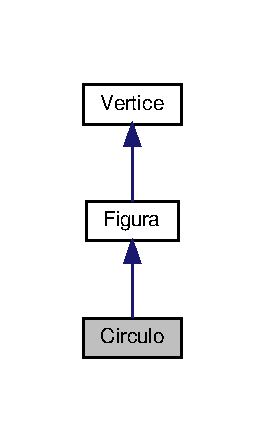
\includegraphics[width=127pt]{class_circulo__inherit__graph}
\end{center}
\end{figure}


Collaboration diagram for Circulo\+:
\nopagebreak
\begin{figure}[H]
\begin{center}
\leavevmode
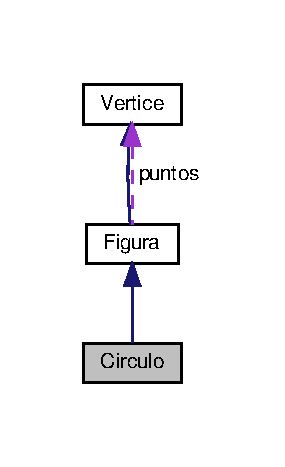
\includegraphics[width=137pt]{class_circulo__coll__graph}
\end{center}
\end{figure}
\subsection*{Public Member Functions}
\begin{DoxyCompactItemize}
\item 
\hyperlink{class_circulo_a790ee75260b927c3b54d534a5d2bab1c}{Circulo} (\hyperlink{class_vertice}{Vertice} $\ast$puntos)
\begin{DoxyCompactList}\small\item\em Constructor de circulo. \end{DoxyCompactList}\item 
\hyperlink{class_circulo_a6ed2ee2a18458c368ab402db2189f60f}{Circulo} (const \hyperlink{class_circulo}{Circulo} \&f)
\begin{DoxyCompactList}\small\item\em constructor por copia \end{DoxyCompactList}\item 
\mbox{\Hypertarget{class_circulo_a8efe39e0e89487519cd802f0738d3bf4}\label{class_circulo_a8efe39e0e89487519cd802f0738d3bf4}} 
\hyperlink{class_circulo_a8efe39e0e89487519cd802f0738d3bf4}{$\sim$\+Circulo} ()
\begin{DoxyCompactList}\small\item\em destructor de la clase \end{DoxyCompactList}\item 
\mbox{\Hypertarget{class_circulo_acc35f8fdd7303fca9fe54b0da458bdf2}\label{class_circulo_acc35f8fdd7303fca9fe54b0da458bdf2}} 
double \hyperlink{class_circulo_acc35f8fdd7303fca9fe54b0da458bdf2}{perimetro} ()
\begin{DoxyCompactList}\small\item\em Calcula el perimetro. \end{DoxyCompactList}\item 
\mbox{\Hypertarget{class_circulo_a12314ab6d649a9e6c1300c6950a46ce7}\label{class_circulo_a12314ab6d649a9e6c1300c6950a46ce7}} 
double \hyperlink{class_circulo_a12314ab6d649a9e6c1300c6950a46ce7}{superficie} ()
\begin{DoxyCompactList}\small\item\em Calcula la superficie. \end{DoxyCompactList}\item 
\mbox{\Hypertarget{class_circulo_ac79dde5c3b5205403a91c694054a3d66}\label{class_circulo_ac79dde5c3b5205403a91c694054a3d66}} 
string \hyperlink{class_circulo_ac79dde5c3b5205403a91c694054a3d66}{operator$\sim$} ()
\begin{DoxyCompactList}\small\item\em sobrecarga del operador $\sim$ para circulo \end{DoxyCompactList}\end{DoxyCompactItemize}
\subsection*{Public Attributes}
\begin{DoxyCompactItemize}
\item 
\mbox{\Hypertarget{class_circulo_aba57029c5768d344c4ef536e5323122b}\label{class_circulo_aba57029c5768d344c4ef536e5323122b}} 
double {\bfseries radio}
\end{DoxyCompactItemize}
\subsection*{Additional Inherited Members}


\subsection{Detailed Description}
clase que se encarga e modelar un circulo 

\subsection{Constructor \& Destructor Documentation}
\mbox{\Hypertarget{class_circulo_a790ee75260b927c3b54d534a5d2bab1c}\label{class_circulo_a790ee75260b927c3b54d534a5d2bab1c}} 
\index{Circulo@{Circulo}!Circulo@{Circulo}}
\index{Circulo@{Circulo}!Circulo@{Circulo}}
\subsubsection{\texorpdfstring{Circulo()}{Circulo()}\hspace{0.1cm}{\footnotesize\ttfamily [1/2]}}
{\footnotesize\ttfamily Circulo\+::\+Circulo (\begin{DoxyParamCaption}\item[{\hyperlink{class_vertice}{Vertice} $\ast$}]{temp }\end{DoxyParamCaption})}



Constructor de circulo. 


\begin{DoxyParams}{Parameters}
{\em temp} & es un puntero de un arreglo de vertices \\
\hline
\end{DoxyParams}
\mbox{\Hypertarget{class_circulo_a6ed2ee2a18458c368ab402db2189f60f}\label{class_circulo_a6ed2ee2a18458c368ab402db2189f60f}} 
\index{Circulo@{Circulo}!Circulo@{Circulo}}
\index{Circulo@{Circulo}!Circulo@{Circulo}}
\subsubsection{\texorpdfstring{Circulo()}{Circulo()}\hspace{0.1cm}{\footnotesize\ttfamily [2/2]}}
{\footnotesize\ttfamily Circulo\+::\+Circulo (\begin{DoxyParamCaption}\item[{const \hyperlink{class_circulo}{Circulo} \&}]{f }\end{DoxyParamCaption})}



constructor por copia 


\begin{DoxyParams}{Parameters}
{\em f} & es un objeto \\
\hline
\end{DoxyParams}


The documentation for this class was generated from the following files\+:\begin{DoxyCompactItemize}
\item 
include/\hyperlink{_circulo_8hpp}{Circulo.\+hpp}\item 
sourcecode/\hyperlink{_circulo_8cpp}{Circulo.\+cpp}\end{DoxyCompactItemize}

\hypertarget{class_equilatero}{}\section{Equilatero Class Reference}
\label{class_equilatero}\index{Equilatero@{Equilatero}}


calse equilatero  




{\ttfamily \#include $<$Triangulo.\+hpp$>$}



Inheritance diagram for Equilatero\+:
\nopagebreak
\begin{figure}[H]
\begin{center}
\leavevmode
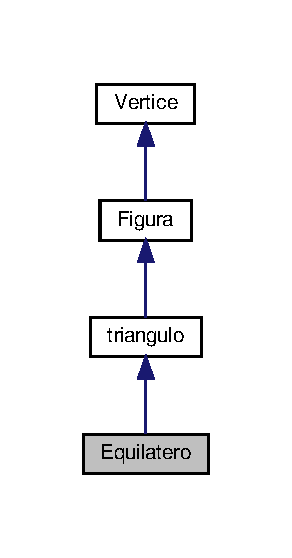
\includegraphics[width=140pt]{class_equilatero__inherit__graph}
\end{center}
\end{figure}


Collaboration diagram for Equilatero\+:
\nopagebreak
\begin{figure}[H]
\begin{center}
\leavevmode
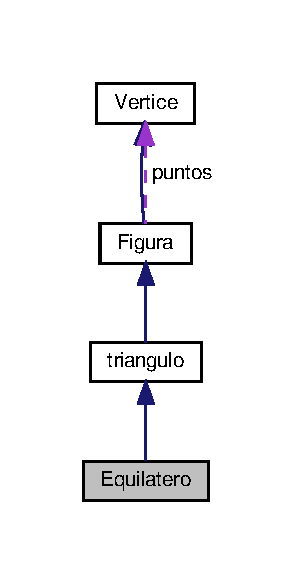
\includegraphics[width=143pt]{class_equilatero__coll__graph}
\end{center}
\end{figure}
\subsection*{Public Member Functions}
\begin{DoxyCompactItemize}
\item 
\hyperlink{class_equilatero_a27bc291f53fa7dfa9a4cc3617bca5ecf}{Equilatero} (\hyperlink{class_vertice}{Vertice} $\ast$puntos)
\begin{DoxyCompactList}\small\item\em Constructor de equilatero. \end{DoxyCompactList}\item 
\hyperlink{class_equilatero_a57d43b4311c0016b838ad9796e9162b4}{Equilatero} (const \hyperlink{class_equilatero}{Equilatero} \&f)
\begin{DoxyCompactList}\small\item\em constructor por copia \end{DoxyCompactList}\item 
\mbox{\Hypertarget{class_equilatero_a16d707c455bde08915f06eeff3a98a99}\label{class_equilatero_a16d707c455bde08915f06eeff3a98a99}} 
double \hyperlink{class_equilatero_a16d707c455bde08915f06eeff3a98a99}{superficie} ()
\begin{DoxyCompactList}\small\item\em calcula la superficie \end{DoxyCompactList}\item 
\mbox{\Hypertarget{class_equilatero_a1e103b1d16b785da9a8b43b17739ad7a}\label{class_equilatero_a1e103b1d16b785da9a8b43b17739ad7a}} 
string \hyperlink{class_equilatero_a1e103b1d16b785da9a8b43b17739ad7a}{operator$\sim$} ()
\begin{DoxyCompactList}\small\item\em sobrecarga del operador $\sim$ para equilatero \end{DoxyCompactList}\end{DoxyCompactItemize}
\subsection*{Additional Inherited Members}


\subsection{Detailed Description}
calse equilatero 

\subsection{Constructor \& Destructor Documentation}
\mbox{\Hypertarget{class_equilatero_a27bc291f53fa7dfa9a4cc3617bca5ecf}\label{class_equilatero_a27bc291f53fa7dfa9a4cc3617bca5ecf}} 
\index{Equilatero@{Equilatero}!Equilatero@{Equilatero}}
\index{Equilatero@{Equilatero}!Equilatero@{Equilatero}}
\subsubsection{\texorpdfstring{Equilatero()}{Equilatero()}\hspace{0.1cm}{\footnotesize\ttfamily [1/2]}}
{\footnotesize\ttfamily Equilatero\+::\+Equilatero (\begin{DoxyParamCaption}\item[{\hyperlink{class_vertice}{Vertice} $\ast$}]{temp }\end{DoxyParamCaption})}



Constructor de equilatero. 


\begin{DoxyParams}{Parameters}
{\em temp} & es un puntero de un arreglo de vertices \\
\hline
\end{DoxyParams}
\mbox{\Hypertarget{class_equilatero_a57d43b4311c0016b838ad9796e9162b4}\label{class_equilatero_a57d43b4311c0016b838ad9796e9162b4}} 
\index{Equilatero@{Equilatero}!Equilatero@{Equilatero}}
\index{Equilatero@{Equilatero}!Equilatero@{Equilatero}}
\subsubsection{\texorpdfstring{Equilatero()}{Equilatero()}\hspace{0.1cm}{\footnotesize\ttfamily [2/2]}}
{\footnotesize\ttfamily Equilatero\+::\+Equilatero (\begin{DoxyParamCaption}\item[{const \hyperlink{class_equilatero}{Equilatero} \&}]{f }\end{DoxyParamCaption})}



constructor por copia 


\begin{DoxyParams}{Parameters}
{\em f} & es un objeto \\
\hline
\end{DoxyParams}


The documentation for this class was generated from the following files\+:\begin{DoxyCompactItemize}
\item 
include/\hyperlink{_triangulo_8hpp}{Triangulo.\+hpp}\item 
sourcecode/\hyperlink{_triangulo_8cpp}{Triangulo.\+cpp}\end{DoxyCompactItemize}

\hypertarget{class_escaleno}{}\section{Escaleno Class Reference}
\label{class_escaleno}\index{Escaleno@{Escaleno}}


calse \hyperlink{class_escaleno}{Escaleno}  




{\ttfamily \#include $<$Triangulo.\+hpp$>$}



Inheritance diagram for Escaleno\+:
\nopagebreak
\begin{figure}[H]
\begin{center}
\leavevmode
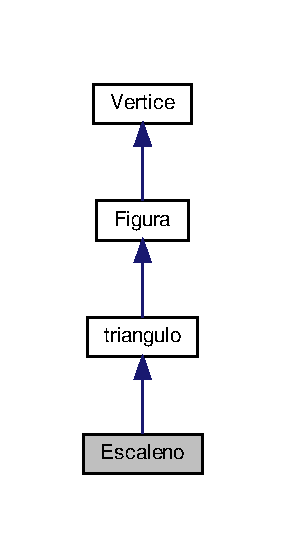
\includegraphics[width=137pt]{class_escaleno__inherit__graph}
\end{center}
\end{figure}


Collaboration diagram for Escaleno\+:
\nopagebreak
\begin{figure}[H]
\begin{center}
\leavevmode
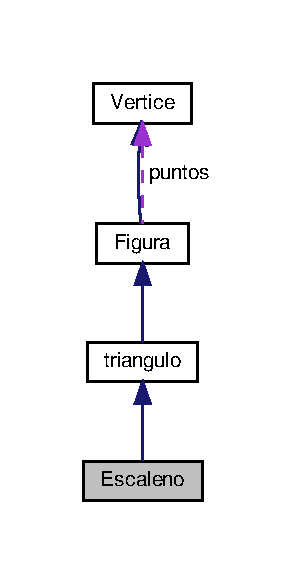
\includegraphics[width=142pt]{class_escaleno__coll__graph}
\end{center}
\end{figure}
\subsection*{Public Member Functions}
\begin{DoxyCompactItemize}
\item 
\hyperlink{class_escaleno_a2670875a1c4940661ea68fb97a8e2da1}{Escaleno} (\hyperlink{class_vertice}{Vertice} $\ast$puntos)
\begin{DoxyCompactList}\small\item\em Constructor de \hyperlink{class_escaleno}{Escaleno}. \end{DoxyCompactList}\item 
\mbox{\Hypertarget{class_escaleno_a49f27943915cf764e133b4ebd24ca060}\label{class_escaleno_a49f27943915cf764e133b4ebd24ca060}} 
\hyperlink{class_escaleno_a49f27943915cf764e133b4ebd24ca060}{$\sim$\+Escaleno} ()
\begin{DoxyCompactList}\small\item\em destructor de \hyperlink{class_escaleno}{Escaleno} \end{DoxyCompactList}\item 
\mbox{\Hypertarget{class_escaleno_a7d71f0f712f7673eca014f1821b78846}\label{class_escaleno_a7d71f0f712f7673eca014f1821b78846}} 
double \hyperlink{class_escaleno_a7d71f0f712f7673eca014f1821b78846}{superficie} ()
\begin{DoxyCompactList}\small\item\em calcula la superficie de un \hyperlink{class_escaleno}{Escaleno} \end{DoxyCompactList}\item 
\mbox{\Hypertarget{class_escaleno_a083472de2f48b2d3da5e11a4d33be38a}\label{class_escaleno_a083472de2f48b2d3da5e11a4d33be38a}} 
string \hyperlink{class_escaleno_a083472de2f48b2d3da5e11a4d33be38a}{operator$\sim$} ()
\begin{DoxyCompactList}\small\item\em sobrecarga del operador $\sim$ para \hyperlink{class_escaleno}{Escaleno} \end{DoxyCompactList}\end{DoxyCompactItemize}
\subsection*{Public Attributes}
\begin{DoxyCompactItemize}
\item 
\mbox{\Hypertarget{class_escaleno_aa7147d8466b9cd87a787a898fed69eec}\label{class_escaleno_aa7147d8466b9cd87a787a898fed69eec}} 
float {\bfseries semiperimetro}
\item 
\mbox{\Hypertarget{class_escaleno_a27961baaa7d8644ca529f200ba968eaa}\label{class_escaleno_a27961baaa7d8644ca529f200ba968eaa}} 
double {\bfseries s}
\end{DoxyCompactItemize}
\subsection*{Additional Inherited Members}


\subsection{Detailed Description}
calse \hyperlink{class_escaleno}{Escaleno} 

Definition at line 28 of file Triangulo.\+hpp.



\subsection{Constructor \& Destructor Documentation}
\mbox{\Hypertarget{class_escaleno_a2670875a1c4940661ea68fb97a8e2da1}\label{class_escaleno_a2670875a1c4940661ea68fb97a8e2da1}} 
\index{Escaleno@{Escaleno}!Escaleno@{Escaleno}}
\index{Escaleno@{Escaleno}!Escaleno@{Escaleno}}
\subsubsection{\texorpdfstring{Escaleno()}{Escaleno()}}
{\footnotesize\ttfamily Escaleno\+::\+Escaleno (\begin{DoxyParamCaption}\item[{\hyperlink{class_vertice}{Vertice} $\ast$}]{temp }\end{DoxyParamCaption})}



Constructor de \hyperlink{class_escaleno}{Escaleno}. 


\begin{DoxyParams}{Parameters}
{\em temp} & es un puntero de un arreglo de vertices \\
\hline
\end{DoxyParams}


Definition at line 106 of file Triangulo.\+cpp.



The documentation for this class was generated from the following files\+:\begin{DoxyCompactItemize}
\item 
/home/jzunigame/\+Documentos/\+A\+\_\+\+Algoritmos/\+A\+\_\+\+Git/\+Laboratorios/\+Lab5 Arboles/reporte/\+Reporte latex/Triangulo.\+hpp\item 
/home/jzunigame/\+Documentos/\+A\+\_\+\+Algoritmos/\+A\+\_\+\+Git/\+Laboratorios/\+Lab5 Arboles/reporte/\+Reporte latex/Triangulo.\+cpp\end{DoxyCompactItemize}

\hypertarget{class_figura}{}\section{Figura Class Reference}
\label{class_figura}\index{Figura@{Figura}}


clase que se encarga de crear una figura en 2D  




{\ttfamily \#include $<$Figura.\+hpp$>$}



Inheritance diagram for Figura\+:
\nopagebreak
\begin{figure}[H]
\begin{center}
\leavevmode
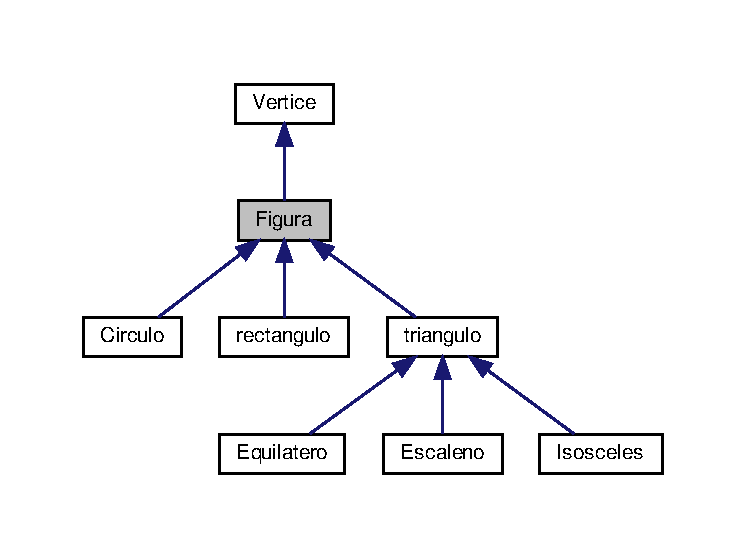
\includegraphics[width=350pt]{class_figura__inherit__graph}
\end{center}
\end{figure}


Collaboration diagram for Figura\+:
\nopagebreak
\begin{figure}[H]
\begin{center}
\leavevmode
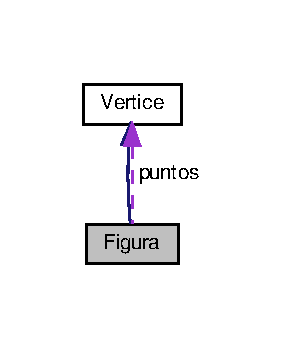
\includegraphics[width=137pt]{class_figura__coll__graph}
\end{center}
\end{figure}
\subsection*{Public Member Functions}
\begin{DoxyCompactItemize}
\item 
\mbox{\Hypertarget{class_figura_a6977c7f0438c11b985a9a74c208b51c8}\label{class_figura_a6977c7f0438c11b985a9a74c208b51c8}} 
\hyperlink{class_figura_a6977c7f0438c11b985a9a74c208b51c8}{Figura} ()
\begin{DoxyCompactList}\small\item\em constructor por defecto \end{DoxyCompactList}\item 
\mbox{\Hypertarget{class_figura_a6130eb548893c36efcb7933e2da6821e}\label{class_figura_a6130eb548893c36efcb7933e2da6821e}} 
\hyperlink{class_figura_a6130eb548893c36efcb7933e2da6821e}{$\sim$\+Figura} ()
\begin{DoxyCompactList}\small\item\em destructor por defecto \end{DoxyCompactList}\item 
\hyperlink{class_figura_a2f55faa2fd40a5ebb2c5d1c958927f2a}{Figura} (const \hyperlink{class_figura}{Figura} \&f)
\begin{DoxyCompactList}\small\item\em constructor por copia \end{DoxyCompactList}\item 
\mbox{\Hypertarget{class_figura_aaaff1d3f33df845278d20b5eab009fca}\label{class_figura_aaaff1d3f33df845278d20b5eab009fca}} 
virtual double \hyperlink{class_figura_aaaff1d3f33df845278d20b5eab009fca}{superficie} ()=0
\begin{DoxyCompactList}\small\item\em metodo que calcula una superficie generica \end{DoxyCompactList}\item 
\mbox{\Hypertarget{class_figura_ad41d892aad534c23be85b96671c09d78}\label{class_figura_ad41d892aad534c23be85b96671c09d78}} 
virtual double \hyperlink{class_figura_ad41d892aad534c23be85b96671c09d78}{perimetro} ()=0
\begin{DoxyCompactList}\small\item\em metodo que calcula un perimetro generico \end{DoxyCompactList}\item 
\mbox{\Hypertarget{class_figura_a56c66abd270dbf126bfb2e8d69b646f6}\label{class_figura_a56c66abd270dbf126bfb2e8d69b646f6}} 
virtual string \hyperlink{class_figura_a56c66abd270dbf126bfb2e8d69b646f6}{operator$\sim$} ()=0
\begin{DoxyCompactList}\small\item\em sobrecarga del operador $\sim$ \end{DoxyCompactList}\end{DoxyCompactItemize}
\subsection*{Public Attributes}
\begin{DoxyCompactItemize}
\item 
\mbox{\Hypertarget{class_figura_ae0b5056c74aade600709487640d5f679}\label{class_figura_ae0b5056c74aade600709487640d5f679}} 
\hyperlink{class_vertice}{Vertice} $\ast$ {\bfseries puntos}
\item 
\mbox{\Hypertarget{class_figura_ae3d1ec3d0d1e9786bb200112a018bc87}\label{class_figura_ae3d1ec3d0d1e9786bb200112a018bc87}} 
float {\bfseries area}
\item 
\mbox{\Hypertarget{class_figura_a261190a959c238f674083daaadb6bd79}\label{class_figura_a261190a959c238f674083daaadb6bd79}} 
float {\bfseries perimetrofig}
\item 
\mbox{\Hypertarget{class_figura_a5be336617ed8a4d4f28115297b38da02}\label{class_figura_a5be336617ed8a4d4f28115297b38da02}} 
string {\bfseries nombre}
\item 
\mbox{\Hypertarget{class_figura_a9f519b9504b95440f124a3099070e952}\label{class_figura_a9f519b9504b95440f124a3099070e952}} 
string {\bfseries color}
\item 
\mbox{\Hypertarget{class_figura_ad45f3e1033b11ecd2205154a7dff6a36}\label{class_figura_ad45f3e1033b11ecd2205154a7dff6a36}} 
int {\bfseries cantidad\+Puntos}
\item 
\mbox{\Hypertarget{class_figura_a29836f970de23e98d29116a0179f8618}\label{class_figura_a29836f970de23e98d29116a0179f8618}} 
string {\bfseries impresion}
\end{DoxyCompactItemize}
\subsection*{Static Public Attributes}
\begin{DoxyCompactItemize}
\item 
\mbox{\Hypertarget{class_figura_a06e9faa5dd891e95a5d4f041e63266b7}\label{class_figura_a06e9faa5dd891e95a5d4f041e63266b7}} 
static int {\bfseries identificador\+Estatico}
\end{DoxyCompactItemize}


\subsection{Detailed Description}
clase que se encarga de crear una figura en 2D 

\subsection{Constructor \& Destructor Documentation}
\mbox{\Hypertarget{class_figura_a2f55faa2fd40a5ebb2c5d1c958927f2a}\label{class_figura_a2f55faa2fd40a5ebb2c5d1c958927f2a}} 
\index{Figura@{Figura}!Figura@{Figura}}
\index{Figura@{Figura}!Figura@{Figura}}
\subsubsection{\texorpdfstring{Figura()}{Figura()}}
{\footnotesize\ttfamily Figura\+::\+Figura (\begin{DoxyParamCaption}\item[{const \hyperlink{class_figura}{Figura} \&}]{f }\end{DoxyParamCaption})}



constructor por copia 


\begin{DoxyParams}{Parameters}
{\em f} & es un objeto \\
\hline
\end{DoxyParams}


The documentation for this class was generated from the following files\+:\begin{DoxyCompactItemize}
\item 
include/\hyperlink{_figura_8hpp}{Figura.\+hpp}\item 
sourcecode/\hyperlink{_figura_8cpp}{Figura.\+cpp}\end{DoxyCompactItemize}

\hypertarget{class_impresora}{}\section{Impresora$<$ T $>$ Class Template Reference}
\label{class_impresora}\index{Impresora$<$ T $>$@{Impresora$<$ T $>$}}


clase que imprmime objetos  




{\ttfamily \#include $<$Impresora.\+hpp$>$}

\subsection*{Public Member Functions}
\begin{DoxyCompactItemize}
\item 
\mbox{\Hypertarget{class_impresora_a68f5ddc334afffb8715f6a6a06ee917b}\label{class_impresora_a68f5ddc334afffb8715f6a6a06ee917b}} 
\hyperlink{class_impresora_a68f5ddc334afffb8715f6a6a06ee917b}{Impresora} ()
\begin{DoxyCompactList}\small\item\em constructor por defecto \end{DoxyCompactList}\item 
\hyperlink{class_impresora_a82093c181cb0601fc82dbbeff7247763}{Impresora} (T fig, string impresion)
\begin{DoxyCompactList}\small\item\em constructor creado mediante template \end{DoxyCompactList}\item 
\mbox{\Hypertarget{class_impresora_a6e8f0ae96313109222fe715137f68b3e}\label{class_impresora_a6e8f0ae96313109222fe715137f68b3e}} 
\hyperlink{class_impresora_a6e8f0ae96313109222fe715137f68b3e}{$\sim$\+Impresora} ()
\begin{DoxyCompactList}\small\item\em destructor por defecto de la clase \end{DoxyCompactList}\item 
string \hyperlink{class_impresora_abab8709ec339f549ef44dae439b33f12}{Obtener\+Color} (string nom\+Color)
\begin{DoxyCompactList}\small\item\em clase que permite imprimir en el color correcto \end{DoxyCompactList}\item 
void \hyperlink{class_impresora_a7427f11d194603c5ae2b7f4837c49f14}{imprimir\+Pantalla} (const T \&objeto)
\begin{DoxyCompactList}\small\item\em metodo que permite imprmir la pantalla \end{DoxyCompactList}\item 
void \hyperlink{class_impresora_ac63e5482787086f73c351732f4731239}{imprimir\+Archivo} (const T \&objeto, string ruta\+Archivo)
\begin{DoxyCompactList}\small\item\em metodo que permite imprmir a un archivo \end{DoxyCompactList}\end{DoxyCompactItemize}
\subsection*{Public Attributes}
\begin{DoxyCompactItemize}
\item 
\mbox{\Hypertarget{class_impresora_a65df8a4e9e23fe2ff39c0b786e833b34}\label{class_impresora_a65df8a4e9e23fe2ff39c0b786e833b34}} 
string {\bfseries ruta}
\end{DoxyCompactItemize}


\subsection{Detailed Description}
\subsubsection*{template$<$class T$>$\newline
class Impresora$<$ T $>$}

clase que imprmime objetos 

\subsection{Constructor \& Destructor Documentation}
\mbox{\Hypertarget{class_impresora_a82093c181cb0601fc82dbbeff7247763}\label{class_impresora_a82093c181cb0601fc82dbbeff7247763}} 
\index{Impresora@{Impresora}!Impresora@{Impresora}}
\index{Impresora@{Impresora}!Impresora@{Impresora}}
\subsubsection{\texorpdfstring{Impresora()}{Impresora()}}
{\footnotesize\ttfamily template$<$class T$>$ \\
\hyperlink{class_impresora}{Impresora}$<$ T $>$\+::\hyperlink{class_impresora}{Impresora} (\begin{DoxyParamCaption}\item[{T}]{fig,  }\item[{string}]{impresion }\end{DoxyParamCaption})\hspace{0.3cm}{\ttfamily [inline]}}



constructor creado mediante template 


\begin{DoxyParams}{Parameters}
{\em fig} & es el objeto recibido por parametro \\
\hline
\end{DoxyParams}


\subsection{Member Function Documentation}
\mbox{\Hypertarget{class_impresora_ac63e5482787086f73c351732f4731239}\label{class_impresora_ac63e5482787086f73c351732f4731239}} 
\index{Impresora@{Impresora}!imprimir\+Archivo@{imprimir\+Archivo}}
\index{imprimir\+Archivo@{imprimir\+Archivo}!Impresora@{Impresora}}
\subsubsection{\texorpdfstring{imprimir\+Archivo()}{imprimirArchivo()}}
{\footnotesize\ttfamily template$<$class T$>$ \\
void \hyperlink{class_impresora}{Impresora}$<$ T $>$\+::imprimir\+Archivo (\begin{DoxyParamCaption}\item[{const T \&}]{objeto,  }\item[{string}]{ruta\+Archivo }\end{DoxyParamCaption})\hspace{0.3cm}{\ttfamily [inline]}}



metodo que permite imprmir a un archivo 


\begin{DoxyParams}{Parameters}
{\em objeto} & es el objeto que debe imprimir \\
\hline
{\em suta\+Archivo} & es la ruta del archivo a escribir \\
\hline
\end{DoxyParams}
\mbox{\Hypertarget{class_impresora_a7427f11d194603c5ae2b7f4837c49f14}\label{class_impresora_a7427f11d194603c5ae2b7f4837c49f14}} 
\index{Impresora@{Impresora}!imprimir\+Pantalla@{imprimir\+Pantalla}}
\index{imprimir\+Pantalla@{imprimir\+Pantalla}!Impresora@{Impresora}}
\subsubsection{\texorpdfstring{imprimir\+Pantalla()}{imprimirPantalla()}}
{\footnotesize\ttfamily template$<$class T$>$ \\
void \hyperlink{class_impresora}{Impresora}$<$ T $>$\+::imprimir\+Pantalla (\begin{DoxyParamCaption}\item[{const T \&}]{objeto }\end{DoxyParamCaption})\hspace{0.3cm}{\ttfamily [inline]}}



metodo que permite imprmir la pantalla 


\begin{DoxyParams}{Parameters}
{\em objeto} & es el objeto que debe imprimir \\
\hline
\end{DoxyParams}
\mbox{\Hypertarget{class_impresora_abab8709ec339f549ef44dae439b33f12}\label{class_impresora_abab8709ec339f549ef44dae439b33f12}} 
\index{Impresora@{Impresora}!Obtener\+Color@{Obtener\+Color}}
\index{Obtener\+Color@{Obtener\+Color}!Impresora@{Impresora}}
\subsubsection{\texorpdfstring{Obtener\+Color()}{ObtenerColor()}}
{\footnotesize\ttfamily template$<$class T$>$ \\
string \hyperlink{class_impresora}{Impresora}$<$ T $>$\+::Obtener\+Color (\begin{DoxyParamCaption}\item[{string}]{nom\+Color }\end{DoxyParamCaption})\hspace{0.3cm}{\ttfamily [inline]}}



clase que permite imprimir en el color correcto 


\begin{DoxyParams}{Parameters}
{\em nom\+Color} & es el color que debe buscar \\
\hline
\end{DoxyParams}
\begin{DoxyReturn}{Returns}
debuelve el codigo de color que debe imprimir 
\end{DoxyReturn}


The documentation for this class was generated from the following file\+:\begin{DoxyCompactItemize}
\item 
include/\hyperlink{_impresora_8hpp}{Impresora.\+hpp}\end{DoxyCompactItemize}

\hypertarget{class_isosceles}{}\section{Isosceles Class Reference}
\label{class_isosceles}\index{Isosceles@{Isosceles}}


calse \hyperlink{class_isosceles}{Isosceles}  




{\ttfamily \#include $<$Triangulo.\+hpp$>$}



Inheritance diagram for Isosceles\+:
\nopagebreak
\begin{figure}[H]
\begin{center}
\leavevmode
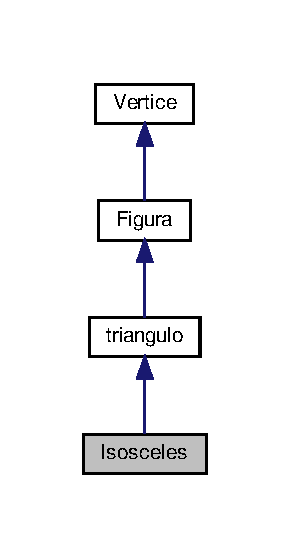
\includegraphics[width=139pt]{class_isosceles__inherit__graph}
\end{center}
\end{figure}


Collaboration diagram for Isosceles\+:
\nopagebreak
\begin{figure}[H]
\begin{center}
\leavevmode
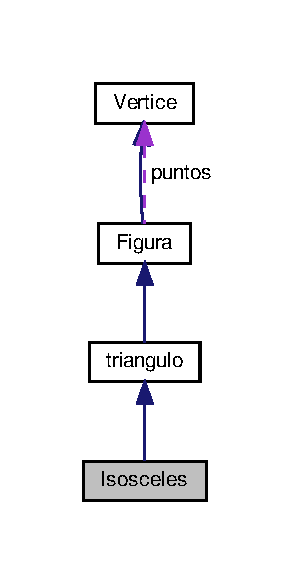
\includegraphics[width=143pt]{class_isosceles__coll__graph}
\end{center}
\end{figure}
\subsection*{Public Member Functions}
\begin{DoxyCompactItemize}
\item 
\hyperlink{class_isosceles_a5dc812e7ac02a71016cdc2175176608a}{Isosceles} (\hyperlink{class_vertice}{Vertice} $\ast$puntos)
\begin{DoxyCompactList}\small\item\em Constructor de \hyperlink{class_isosceles}{Isosceles}. \end{DoxyCompactList}\item 
\hyperlink{class_isosceles_a7190cc477e9835205f3061633f73825f}{Isosceles} (const \hyperlink{class_isosceles}{Isosceles} \&f)
\begin{DoxyCompactList}\small\item\em constructor por copia \end{DoxyCompactList}\item 
\mbox{\Hypertarget{class_isosceles_aa09c863c5ef3620e9c57b09ee380d3d1}\label{class_isosceles_aa09c863c5ef3620e9c57b09ee380d3d1}} 
double \hyperlink{class_isosceles_aa09c863c5ef3620e9c57b09ee380d3d1}{superficie} ()
\begin{DoxyCompactList}\small\item\em calcula la superficie \end{DoxyCompactList}\item 
\mbox{\Hypertarget{class_isosceles_a8998981f4d303e909964dfe90f77f445}\label{class_isosceles_a8998981f4d303e909964dfe90f77f445}} 
string \hyperlink{class_isosceles_a8998981f4d303e909964dfe90f77f445}{operator$\sim$} ()
\begin{DoxyCompactList}\small\item\em sobrecarga del operador $\sim$ para \hyperlink{class_isosceles}{Isosceles} \end{DoxyCompactList}\end{DoxyCompactItemize}
\subsection*{Additional Inherited Members}


\subsection{Detailed Description}
calse \hyperlink{class_isosceles}{Isosceles} 

\subsection{Constructor \& Destructor Documentation}
\mbox{\Hypertarget{class_isosceles_a5dc812e7ac02a71016cdc2175176608a}\label{class_isosceles_a5dc812e7ac02a71016cdc2175176608a}} 
\index{Isosceles@{Isosceles}!Isosceles@{Isosceles}}
\index{Isosceles@{Isosceles}!Isosceles@{Isosceles}}
\subsubsection{\texorpdfstring{Isosceles()}{Isosceles()}\hspace{0.1cm}{\footnotesize\ttfamily [1/2]}}
{\footnotesize\ttfamily Isosceles\+::\+Isosceles (\begin{DoxyParamCaption}\item[{\hyperlink{class_vertice}{Vertice} $\ast$}]{temp }\end{DoxyParamCaption})}



Constructor de \hyperlink{class_isosceles}{Isosceles}. 


\begin{DoxyParams}{Parameters}
{\em temp} & es un puntero de un arreglo de vertices \\
\hline
\end{DoxyParams}
\mbox{\Hypertarget{class_isosceles_a7190cc477e9835205f3061633f73825f}\label{class_isosceles_a7190cc477e9835205f3061633f73825f}} 
\index{Isosceles@{Isosceles}!Isosceles@{Isosceles}}
\index{Isosceles@{Isosceles}!Isosceles@{Isosceles}}
\subsubsection{\texorpdfstring{Isosceles()}{Isosceles()}\hspace{0.1cm}{\footnotesize\ttfamily [2/2]}}
{\footnotesize\ttfamily Isosceles\+::\+Isosceles (\begin{DoxyParamCaption}\item[{const \hyperlink{class_isosceles}{Isosceles} \&}]{f }\end{DoxyParamCaption})}



constructor por copia 


\begin{DoxyParams}{Parameters}
{\em f} & es un objeto \\
\hline
\end{DoxyParams}


The documentation for this class was generated from the following files\+:\begin{DoxyCompactItemize}
\item 
include/\hyperlink{_triangulo_8hpp}{Triangulo.\+hpp}\item 
sourcecode/\hyperlink{_triangulo_8cpp}{Triangulo.\+cpp}\end{DoxyCompactItemize}

\hypertarget{class_principal}{}\section{Principal Class Reference}
\label{class_principal}\index{Principal@{Principal}}
\subsection*{Public Member Functions}
\begin{DoxyCompactItemize}
\item 
\mbox{\Hypertarget{class_principal_a99454861dd40e945772f9663be9a41ab}\label{class_principal_a99454861dd40e945772f9663be9a41ab}} 
void \hyperlink{class_principal_a99454861dd40e945772f9663be9a41ab}{Bienvenido} ()
\begin{DoxyCompactList}\small\item\em metodo que imprime un banner de bienvenida \end{DoxyCompactList}\item 
\mbox{\Hypertarget{class_principal_a4602cdbef58d0b43a9843df7afca4716}\label{class_principal_a4602cdbef58d0b43a9843df7afca4716}} 
void \hyperlink{class_principal_a4602cdbef58d0b43a9843df7afca4716}{Menu} ()
\begin{DoxyCompactList}\small\item\em metodo que imprime un un menu \end{DoxyCompactList}\item 
void \hyperlink{class_principal_aca941b071da80e6d5202010165950101}{Hacer\+Arreglo\+Vertices} (int cantidad, \hyperlink{class_vertice}{Vertice} $\ast$arreglo)
\begin{DoxyCompactList}\small\item\em metodo que crea un arreglo de objetos tipo vertice \end{DoxyCompactList}\item 
\mbox{\Hypertarget{class_principal_a237db058cac2f5ea38eba6539cde454c}\label{class_principal_a237db058cac2f5ea38eba6539cde454c}} 
string \hyperlink{class_principal_a237db058cac2f5ea38eba6539cde454c}{Color} ()
\begin{DoxyCompactList}\small\item\em metodo que permite escoger un color de figura \end{DoxyCompactList}\item 
\mbox{\Hypertarget{class_principal_a0abea85aebda36925208a3fda0f41c15}\label{class_principal_a0abea85aebda36925208a3fda0f41c15}} 
void \hyperlink{class_principal_a0abea85aebda36925208a3fda0f41c15}{Mtd\+Rectangulo} ()
\begin{DoxyCompactList}\small\item\em metodo que instancia un objeto de tipo rectangulo \end{DoxyCompactList}\item 
\mbox{\Hypertarget{class_principal_a8711ee7dd8bb46d4014a6d27275ea104}\label{class_principal_a8711ee7dd8bb46d4014a6d27275ea104}} 
void \hyperlink{class_principal_a8711ee7dd8bb46d4014a6d27275ea104}{Mtd\+Circulo} ()
\begin{DoxyCompactList}\small\item\em metodo que instancia un objeto de tipo \hyperlink{class_circulo}{Circulo} \end{DoxyCompactList}\item 
\mbox{\Hypertarget{class_principal_afc5a6c41795be6c9c29e4be5c4188322}\label{class_principal_afc5a6c41795be6c9c29e4be5c4188322}} 
void \hyperlink{class_principal_afc5a6c41795be6c9c29e4be5c4188322}{Mtd\+Triangulo} ()
\begin{DoxyCompactList}\small\item\em metodo que instancia un objeto de tipo Triangulo \end{DoxyCompactList}\item 
\mbox{\Hypertarget{class_principal_a3eda271bf0f7f3cc694dd0d6b7a6bc0d}\label{class_principal_a3eda271bf0f7f3cc694dd0d6b7a6bc0d}} 
void \hyperlink{class_principal_a3eda271bf0f7f3cc694dd0d6b7a6bc0d}{Mtd\+Cualquier\+Figura} ()
\begin{DoxyCompactList}\small\item\em metodo que instancia un objeto n cantidad de ladoso \end{DoxyCompactList}\end{DoxyCompactItemize}


\subsection{Member Function Documentation}
\mbox{\Hypertarget{class_principal_aca941b071da80e6d5202010165950101}\label{class_principal_aca941b071da80e6d5202010165950101}} 
\index{Principal@{Principal}!Hacer\+Arreglo\+Vertices@{Hacer\+Arreglo\+Vertices}}
\index{Hacer\+Arreglo\+Vertices@{Hacer\+Arreglo\+Vertices}!Principal@{Principal}}
\subsubsection{\texorpdfstring{Hacer\+Arreglo\+Vertices()}{HacerArregloVertices()}}
{\footnotesize\ttfamily void Principal\+::\+Hacer\+Arreglo\+Vertices (\begin{DoxyParamCaption}\item[{int}]{cantidad,  }\item[{\hyperlink{class_vertice}{Vertice} $\ast$}]{arreglo }\end{DoxyParamCaption})\hspace{0.3cm}{\ttfamily [inline]}}



metodo que crea un arreglo de objetos tipo vertice 


\begin{DoxyParams}{Parameters}
{\em cantidad} & es el numero de vertices \\
\hline
{\em arreglo} & es el puntero del arreglo que se va a pasar \\
\hline
\end{DoxyParams}


The documentation for this class was generated from the following file\+:\begin{DoxyCompactItemize}
\item 
include/\hyperlink{_tools_8hpp}{Tools.\+hpp}\end{DoxyCompactItemize}

\hypertarget{classrectangulo}{}\section{rectangulo Class Reference}
\label{classrectangulo}\index{rectangulo@{rectangulo}}


Clase rectangulo.  




{\ttfamily \#include $<$Rectangulo.\+hpp$>$}



Inheritance diagram for rectangulo\+:
\nopagebreak
\begin{figure}[H]
\begin{center}
\leavevmode
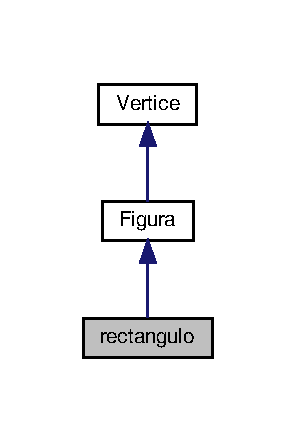
\includegraphics[width=142pt]{classrectangulo__inherit__graph}
\end{center}
\end{figure}


Collaboration diagram for rectangulo\+:
\nopagebreak
\begin{figure}[H]
\begin{center}
\leavevmode
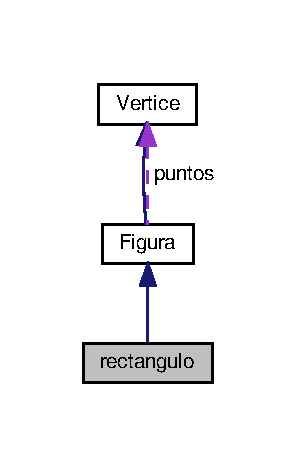
\includegraphics[width=164pt]{classrectangulo__coll__graph}
\end{center}
\end{figure}
\subsection*{Public Member Functions}
\begin{DoxyCompactItemize}
\item 
\hyperlink{classrectangulo_aa785cc2d5bd4cbae7dab1912afba62a7}{rectangulo} (\hyperlink{class_vertice}{Vertice} $\ast$puntos)
\begin{DoxyCompactList}\small\item\em contructor de la clase rectangulo \end{DoxyCompactList}\item 
\mbox{\Hypertarget{classrectangulo_aba192e636fe037aaf0ccc294e4570b29}\label{classrectangulo_aba192e636fe037aaf0ccc294e4570b29}} 
\hyperlink{classrectangulo_aba192e636fe037aaf0ccc294e4570b29}{$\sim$rectangulo} ()
\begin{DoxyCompactList}\small\item\em destructor de la clase \end{DoxyCompactList}\item 
\mbox{\Hypertarget{classrectangulo_ab0db7c753485200cf2577532af506426}\label{classrectangulo_ab0db7c753485200cf2577532af506426}} 
double \hyperlink{classrectangulo_ab0db7c753485200cf2577532af506426}{superficie} ()
\begin{DoxyCompactList}\small\item\em Calcula la superficie. \end{DoxyCompactList}\item 
\mbox{\Hypertarget{classrectangulo_a23a8d0d8a593f80776b4629c6dc435e0}\label{classrectangulo_a23a8d0d8a593f80776b4629c6dc435e0}} 
double \hyperlink{classrectangulo_a23a8d0d8a593f80776b4629c6dc435e0}{perimetro} ()
\begin{DoxyCompactList}\small\item\em Calcula el perimetro. \end{DoxyCompactList}\item 
\mbox{\Hypertarget{classrectangulo_a72992eaf78fb4834cbe2774604a70a0d}\label{classrectangulo_a72992eaf78fb4834cbe2774604a70a0d}} 
string \hyperlink{classrectangulo_a72992eaf78fb4834cbe2774604a70a0d}{operator$\sim$} ()
\begin{DoxyCompactList}\small\item\em sobrecarga del operador $\sim$ para circulo \end{DoxyCompactList}\item 
\mbox{\Hypertarget{classrectangulo_ab0db7c753485200cf2577532af506426}\label{classrectangulo_ab0db7c753485200cf2577532af506426}} 
double \hyperlink{classrectangulo_ab0db7c753485200cf2577532af506426}{superficie} ()
\begin{DoxyCompactList}\small\item\em metodo que calcula una superficie generica \end{DoxyCompactList}\item 
\mbox{\Hypertarget{classrectangulo_a23a8d0d8a593f80776b4629c6dc435e0}\label{classrectangulo_a23a8d0d8a593f80776b4629c6dc435e0}} 
double \hyperlink{classrectangulo_a23a8d0d8a593f80776b4629c6dc435e0}{perimetro} ()
\begin{DoxyCompactList}\small\item\em metodo que calcula un perimetro generico \end{DoxyCompactList}\end{DoxyCompactItemize}
\subsection*{Public Attributes}
\begin{DoxyCompactItemize}
\item 
\mbox{\Hypertarget{classrectangulo_a4793bfe1636488ed8344a82a271dcd8d}\label{classrectangulo_a4793bfe1636488ed8344a82a271dcd8d}} 
float {\bfseries altura}
\item 
\mbox{\Hypertarget{classrectangulo_a0f5bab44f86d9b58bd1c4710f3e001b5}\label{classrectangulo_a0f5bab44f86d9b58bd1c4710f3e001b5}} 
float {\bfseries base}
\end{DoxyCompactItemize}
\subsection*{Additional Inherited Members}


\subsection{Detailed Description}
Clase rectangulo. 

\subsection{Constructor \& Destructor Documentation}
\mbox{\Hypertarget{classrectangulo_aa785cc2d5bd4cbae7dab1912afba62a7}\label{classrectangulo_aa785cc2d5bd4cbae7dab1912afba62a7}} 
\index{rectangulo@{rectangulo}!rectangulo@{rectangulo}}
\index{rectangulo@{rectangulo}!rectangulo@{rectangulo}}
\subsubsection{\texorpdfstring{rectangulo()}{rectangulo()}}
{\footnotesize\ttfamily rectangulo\+::rectangulo (\begin{DoxyParamCaption}\item[{\hyperlink{class_vertice}{Vertice} $\ast$}]{temp }\end{DoxyParamCaption})}



contructor de la clase rectangulo 


\begin{DoxyParams}{Parameters}
{\em recibe} & un puntero a los vertices \\
\hline
\end{DoxyParams}


The documentation for this class was generated from the following files\+:\begin{DoxyCompactItemize}
\item 
include/Rectangulo.\+hpp\item 
reporte/codigo\+Fuente/Rectangulo.\+cpp\end{DoxyCompactItemize}

\hypertarget{classtriangulo}{}\section{triangulo Class Reference}
\label{classtriangulo}\index{triangulo@{triangulo}}


calse tringulo  




{\ttfamily \#include $<$Triangulo.\+hpp$>$}



Inheritance diagram for triangulo\+:
\nopagebreak
\begin{figure}[H]
\begin{center}
\leavevmode
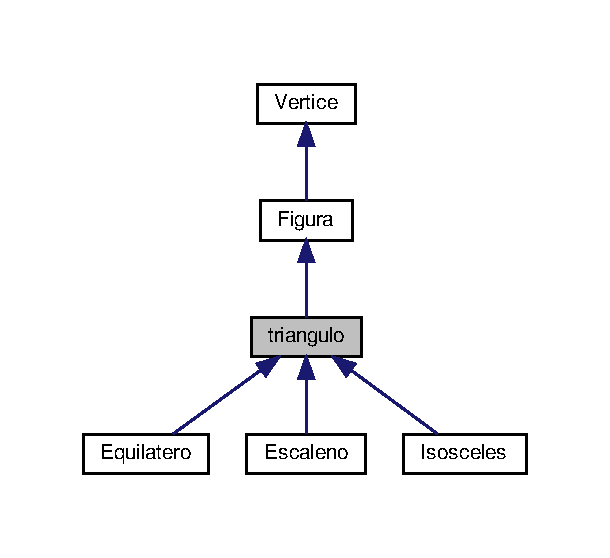
\includegraphics[width=293pt]{classtriangulo__inherit__graph}
\end{center}
\end{figure}


Collaboration diagram for triangulo\+:
\nopagebreak
\begin{figure}[H]
\begin{center}
\leavevmode
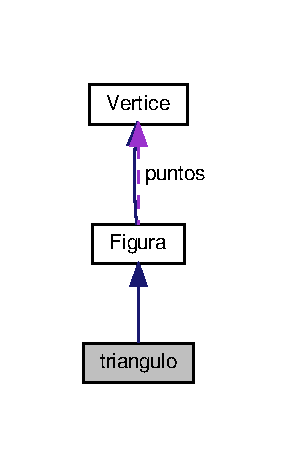
\includegraphics[width=160pt]{classtriangulo__coll__graph}
\end{center}
\end{figure}
\subsection*{Public Member Functions}
\begin{DoxyCompactItemize}
\item 
\mbox{\Hypertarget{classtriangulo_acf725d8856047c7f34f3cc120845d61f}\label{classtriangulo_acf725d8856047c7f34f3cc120845d61f}} 
\hyperlink{classtriangulo_acf725d8856047c7f34f3cc120845d61f}{triangulo} ()
\begin{DoxyCompactList}\small\item\em Constructor de tringulo. \end{DoxyCompactList}\item 
\mbox{\Hypertarget{classtriangulo_a8af9d6bbfd02ed3a82bd30147958ac34}\label{classtriangulo_a8af9d6bbfd02ed3a82bd30147958ac34}} 
\hyperlink{classtriangulo_a8af9d6bbfd02ed3a82bd30147958ac34}{$\sim$triangulo} ()
\begin{DoxyCompactList}\small\item\em Destructor de tringulo. \end{DoxyCompactList}\item 
\mbox{\Hypertarget{classtriangulo_a3e689f3bb9dad9e17766aa2adb060c16}\label{classtriangulo_a3e689f3bb9dad9e17766aa2adb060c16}} 
double \hyperlink{classtriangulo_a3e689f3bb9dad9e17766aa2adb060c16}{perimetro} ()
\begin{DoxyCompactList}\small\item\em metodo que calcula un perimetro generico \end{DoxyCompactList}\item 
\mbox{\Hypertarget{classtriangulo_a21620f40b213174d311380b0343777cb}\label{classtriangulo_a21620f40b213174d311380b0343777cb}} 
virtual string \hyperlink{classtriangulo_a21620f40b213174d311380b0343777cb}{operator$\sim$} ()
\begin{DoxyCompactList}\small\item\em sobrecarga del operador $\sim$ para trinagulo \end{DoxyCompactList}\item 
\mbox{\Hypertarget{classtriangulo_a3e689f3bb9dad9e17766aa2adb060c16}\label{classtriangulo_a3e689f3bb9dad9e17766aa2adb060c16}} 
double \hyperlink{classtriangulo_a3e689f3bb9dad9e17766aa2adb060c16}{perimetro} ()
\begin{DoxyCompactList}\small\item\em metodo que calcula un perimetro generico \end{DoxyCompactList}\end{DoxyCompactItemize}
\subsection*{Public Attributes}
\begin{DoxyCompactItemize}
\item 
\mbox{\Hypertarget{classtriangulo_a938be48c572df73b6cc2aa18f83b83c4}\label{classtriangulo_a938be48c572df73b6cc2aa18f83b83c4}} 
float {\bfseries lado1}
\item 
\mbox{\Hypertarget{classtriangulo_ab4441e41406099469c085abb287f9b8c}\label{classtriangulo_ab4441e41406099469c085abb287f9b8c}} 
float {\bfseries lado2}
\item 
\mbox{\Hypertarget{classtriangulo_aff3acd0f532f7c2e8bac5c2709124433}\label{classtriangulo_aff3acd0f532f7c2e8bac5c2709124433}} 
float {\bfseries lado3}
\item 
\mbox{\Hypertarget{classtriangulo_aacb96b1b6b60488b47bfcd422e0530ba}\label{classtriangulo_aacb96b1b6b60488b47bfcd422e0530ba}} 
bool {\bfseries equilatero} =false
\end{DoxyCompactItemize}
\subsection*{Additional Inherited Members}


\subsection{Detailed Description}
calse tringulo 

The documentation for this class was generated from the following files\+:\begin{DoxyCompactItemize}
\item 
include/Triangulo.\+hpp\item 
reporte/codigo\+Fuente/Triangulo.\+cpp\end{DoxyCompactItemize}

\hypertarget{class_vertice}{}\section{Vertice Class Reference}
\label{class_vertice}\index{Vertice@{Vertice}}


clase que modela un punto en el espacio  




{\ttfamily \#include $<$Vertice.\+hpp$>$}



Inheritance diagram for Vertice\+:
\nopagebreak
\begin{figure}[H]
\begin{center}
\leavevmode
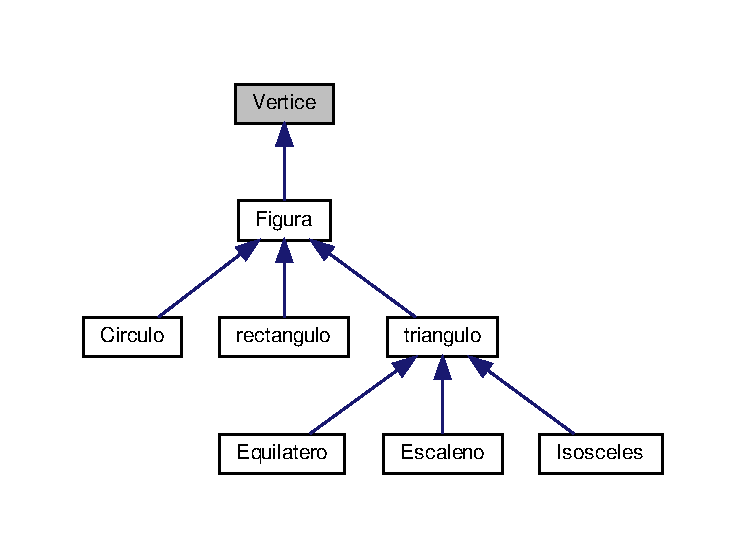
\includegraphics[width=350pt]{class_vertice__inherit__graph}
\end{center}
\end{figure}
\subsection*{Public Member Functions}
\begin{DoxyCompactItemize}
\item 
\mbox{\Hypertarget{class_vertice_a9dd7cf987cddf248b9d4e3d31bf8822b}\label{class_vertice_a9dd7cf987cddf248b9d4e3d31bf8822b}} 
\hyperlink{class_vertice_a9dd7cf987cddf248b9d4e3d31bf8822b}{Vertice} ()
\begin{DoxyCompactList}\small\item\em constructor por defecto \end{DoxyCompactList}\item 
\mbox{\Hypertarget{class_vertice_ae231694dc3ff35959b5b20b879b4678a}\label{class_vertice_ae231694dc3ff35959b5b20b879b4678a}} 
\hyperlink{class_vertice_ae231694dc3ff35959b5b20b879b4678a}{$\sim$\+Vertice} ()
\begin{DoxyCompactList}\small\item\em desconstructor por defecto \end{DoxyCompactList}\item 
\hyperlink{class_vertice_a8d8f3610b706a9e5d50e1138d9abea90}{Vertice} (const \hyperlink{class_vertice}{Vertice} \&v)
\begin{DoxyCompactList}\small\item\em constructor por copia \end{DoxyCompactList}\item 
\mbox{\Hypertarget{class_vertice_a3c83f2d25882d03116afbc39906bbf31}\label{class_vertice_a3c83f2d25882d03116afbc39906bbf31}} 
string \hyperlink{class_vertice_a3c83f2d25882d03116afbc39906bbf31}{operator$\sim$} ()
\begin{DoxyCompactList}\small\item\em sobrecarga operador $\sim$ para convertir a texto \end{DoxyCompactList}\item 
\mbox{\Hypertarget{class_vertice_a8bf2ff926bc43cba6342d9f57f930708}\label{class_vertice_a8bf2ff926bc43cba6342d9f57f930708}} 
double \hyperlink{class_vertice_a8bf2ff926bc43cba6342d9f57f930708}{operator$>$$>$} (const \hyperlink{class_vertice}{Vertice} \&rhs)
\begin{DoxyCompactList}\small\item\em sobrecarga operador $\sim$ para convertir a texto \end{DoxyCompactList}\end{DoxyCompactItemize}
\subsection*{Public Attributes}
\begin{DoxyCompactItemize}
\item 
\mbox{\Hypertarget{class_vertice_abc7f97df103b9c53bf04e1c6f247c1fc}\label{class_vertice_abc7f97df103b9c53bf04e1c6f247c1fc}} 
float {\bfseries x}
\item 
\mbox{\Hypertarget{class_vertice_aca05e79646b79df75ccf73f07b04d26e}\label{class_vertice_aca05e79646b79df75ccf73f07b04d26e}} 
float {\bfseries y}
\item 
\mbox{\Hypertarget{class_vertice_a923a1c1451729f490b42bbe35bdf20f1}\label{class_vertice_a923a1c1451729f490b42bbe35bdf20f1}} 
int {\bfseries identificador}
\end{DoxyCompactItemize}


\subsection{Detailed Description}
clase que modela un punto en el espacio 

Definition at line 11 of file Vertice.\+hpp.



\subsection{Constructor \& Destructor Documentation}
\mbox{\Hypertarget{class_vertice_a8d8f3610b706a9e5d50e1138d9abea90}\label{class_vertice_a8d8f3610b706a9e5d50e1138d9abea90}} 
\index{Vertice@{Vertice}!Vertice@{Vertice}}
\index{Vertice@{Vertice}!Vertice@{Vertice}}
\subsubsection{\texorpdfstring{Vertice()}{Vertice()}}
{\footnotesize\ttfamily Vertice\+::\+Vertice (\begin{DoxyParamCaption}\item[{const \hyperlink{class_vertice}{Vertice} \&}]{v }\end{DoxyParamCaption})}



constructor por copia 


\begin{DoxyParams}{Parameters}
{\em v} & es un objeto \\
\hline
\end{DoxyParams}


Definition at line 18 of file Vertice.\+cpp.



The documentation for this class was generated from the following files\+:\begin{DoxyCompactItemize}
\item 
/home/jzunigame/\+Documentos/\+A\+\_\+\+Algoritmos/\+A\+\_\+\+Git/\+Laboratorios/\+Lab5 Arboles/reporte/\+Reporte latex/Vertice.\+hpp\item 
/home/jzunigame/\+Documentos/\+A\+\_\+\+Algoritmos/\+A\+\_\+\+Git/\+Laboratorios/\+Lab5 Arboles/reporte/\+Reporte latex/Vertice.\+cpp\end{DoxyCompactItemize}

\chapter{File Documentation}
\hypertarget{_circulo_8hpp}{}\section{include/\+Circulo.hpp File Reference}
\label{_circulo_8hpp}\index{include/\+Circulo.\+hpp@{include/\+Circulo.\+hpp}}
{\ttfamily \#include \char`\"{}./\+Includes.\+hpp\char`\"{}}\newline
Include dependency graph for Circulo.\+hpp\+:
\nopagebreak
\begin{figure}[H]
\begin{center}
\leavevmode
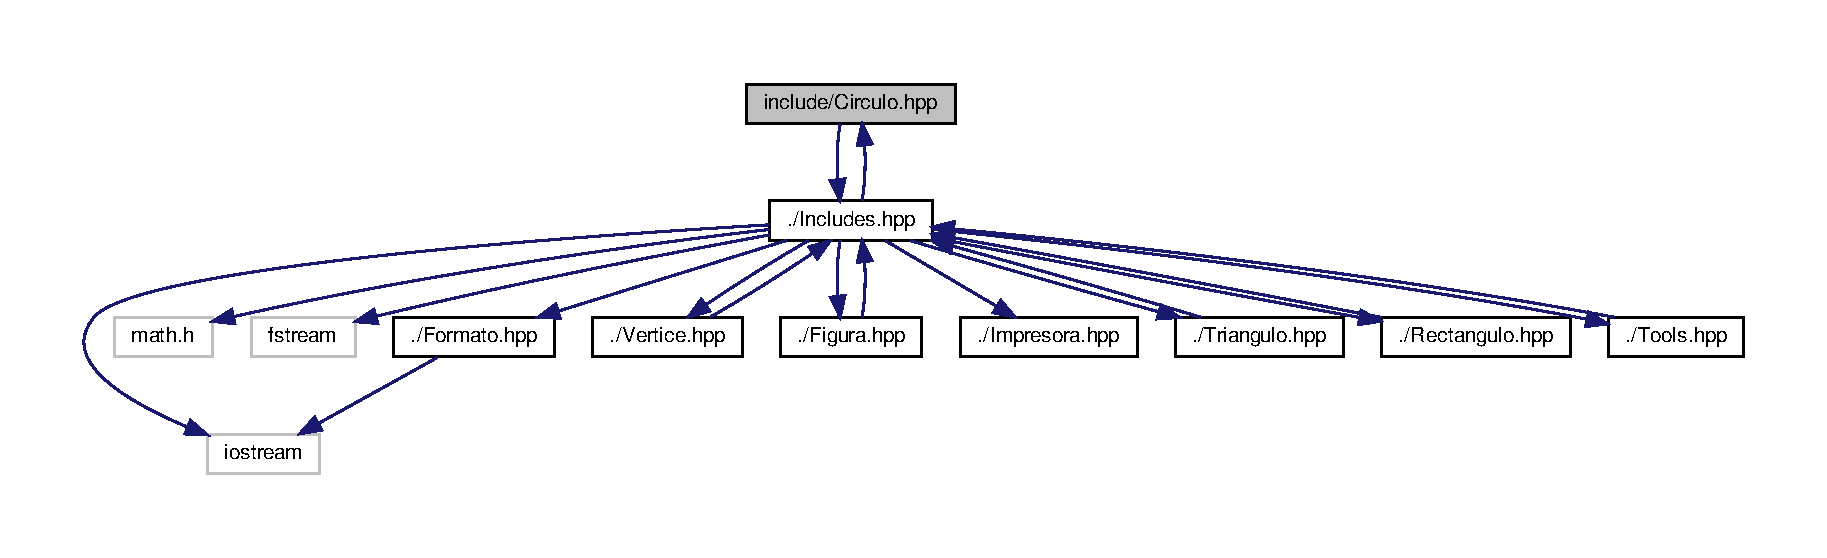
\includegraphics[width=350pt]{_circulo_8hpp__incl}
\end{center}
\end{figure}
This graph shows which files directly or indirectly include this file\+:
\nopagebreak
\begin{figure}[H]
\begin{center}
\leavevmode
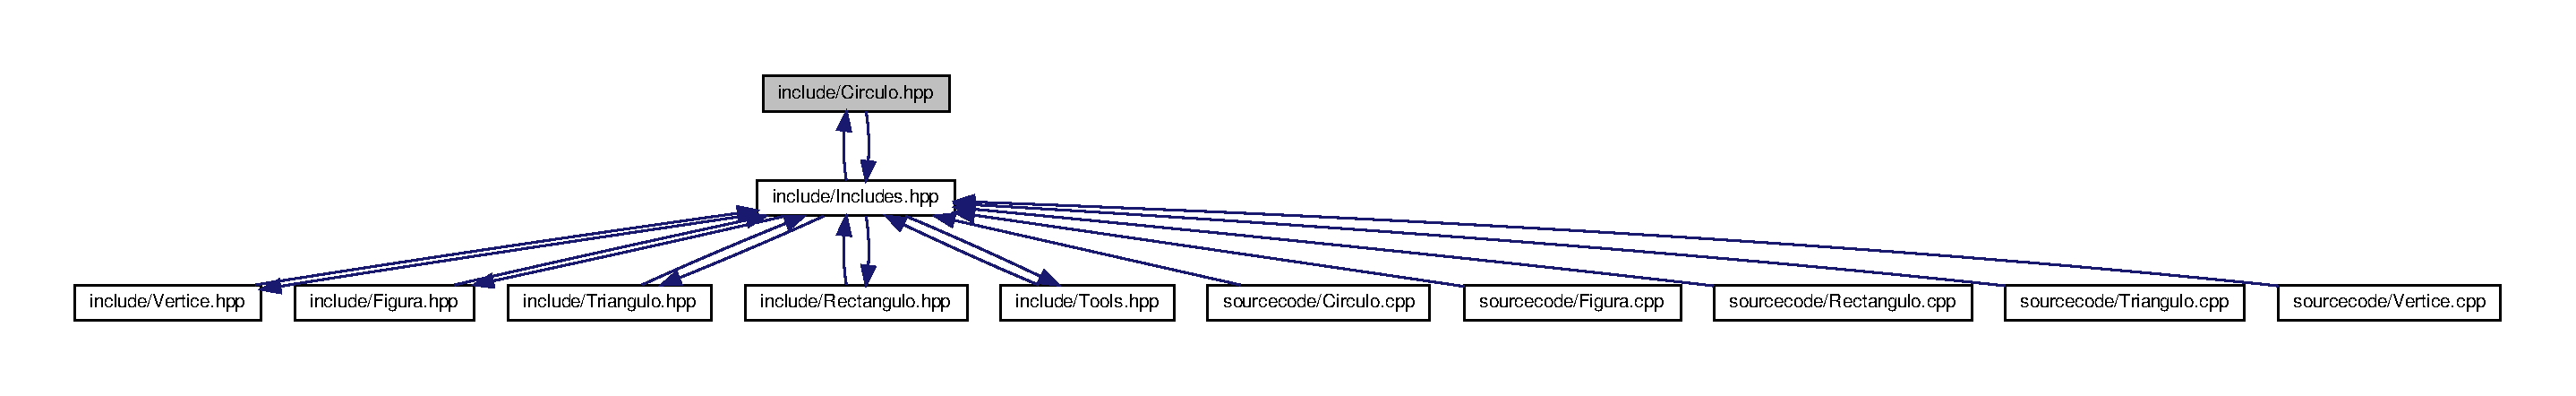
\includegraphics[width=350pt]{_circulo_8hpp__dep__incl}
\end{center}
\end{figure}
\subsection*{Classes}
\begin{DoxyCompactItemize}
\item 
class \hyperlink{class_circulo}{Circulo}
\begin{DoxyCompactList}\small\item\em clase que se encarga e modelar un circulo \end{DoxyCompactList}\end{DoxyCompactItemize}


\subsection{Detailed Description}
/ 
\hypertarget{_figura_8hpp}{}\section{include/\+Figura.hpp File Reference}
\label{_figura_8hpp}\index{include/\+Figura.\+hpp@{include/\+Figura.\+hpp}}
{\ttfamily \#include \char`\"{}./\+Includes.\+hpp\char`\"{}}\newline
Include dependency graph for Figura.\+hpp\+:
\nopagebreak
\begin{figure}[H]
\begin{center}
\leavevmode
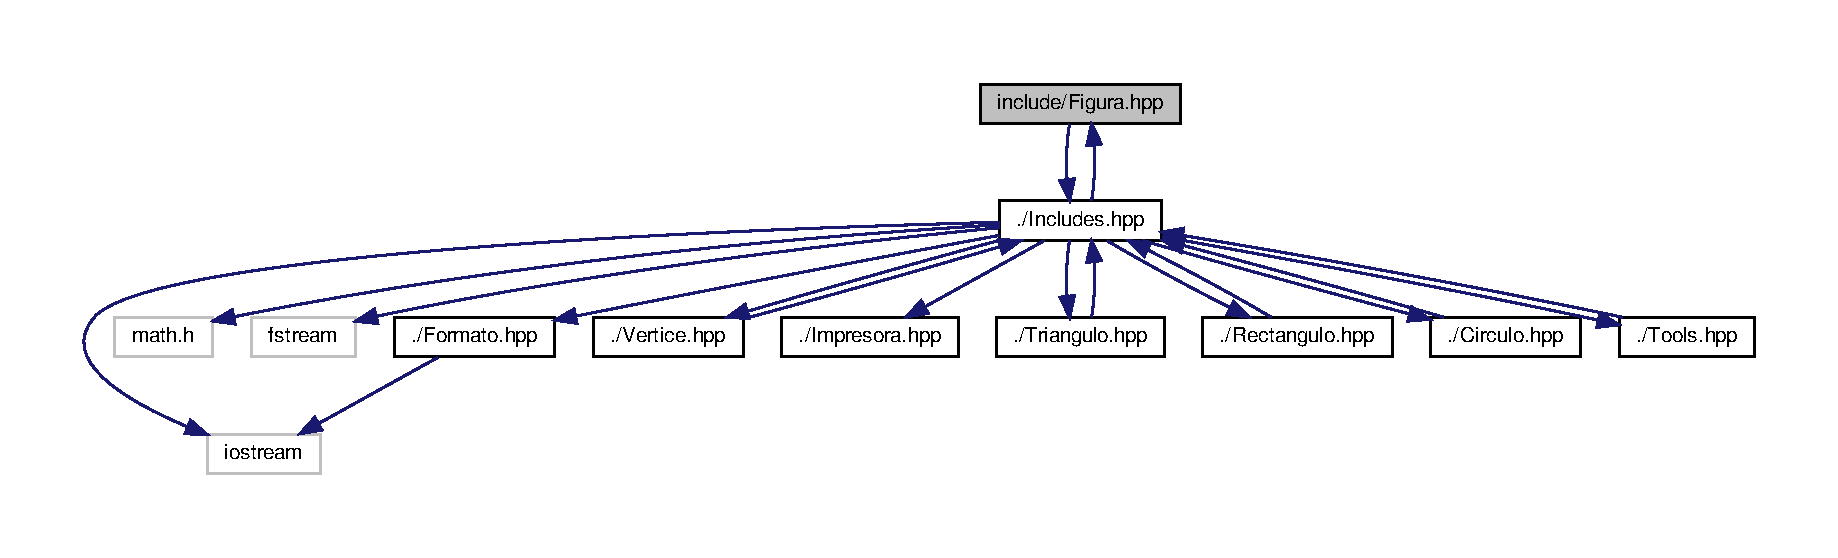
\includegraphics[width=350pt]{_figura_8hpp__incl}
\end{center}
\end{figure}
This graph shows which files directly or indirectly include this file\+:
\nopagebreak
\begin{figure}[H]
\begin{center}
\leavevmode
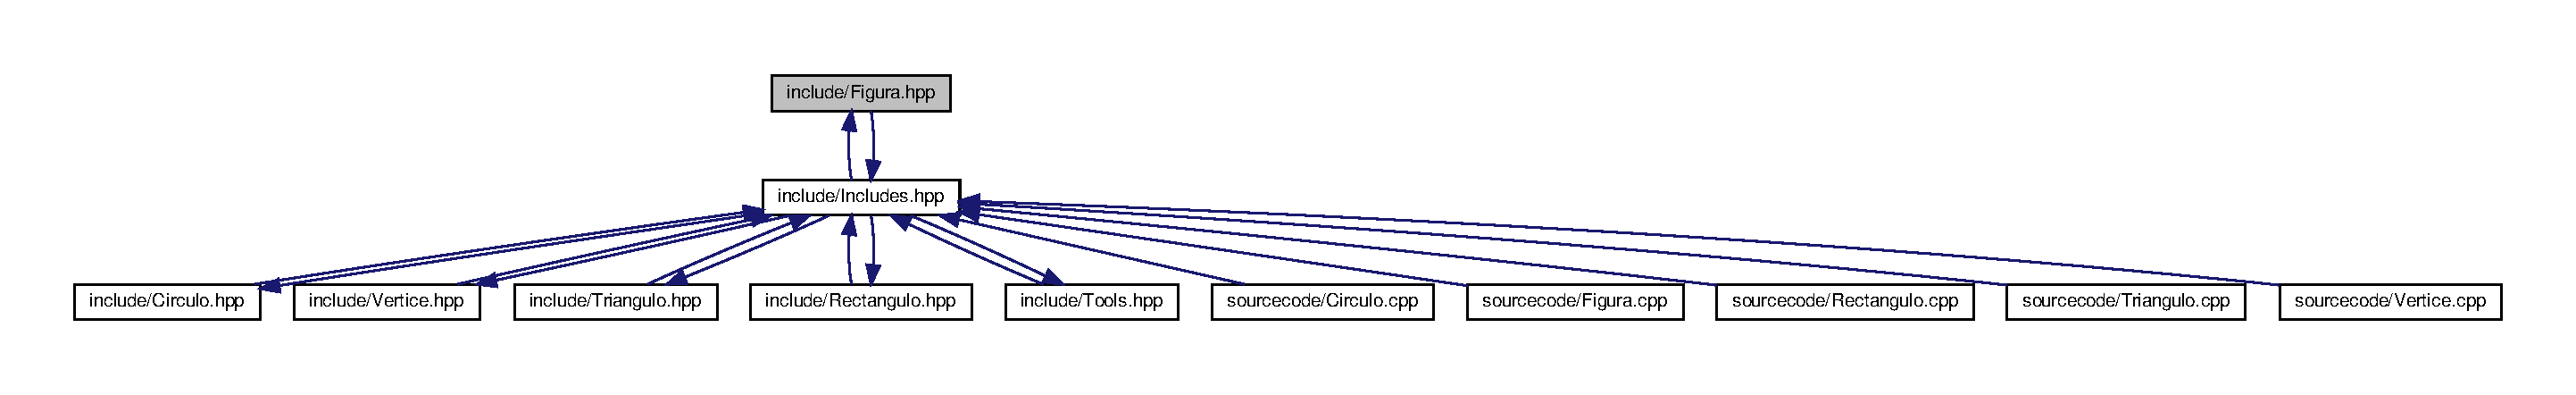
\includegraphics[width=350pt]{_figura_8hpp__dep__incl}
\end{center}
\end{figure}
\subsection*{Classes}
\begin{DoxyCompactItemize}
\item 
class \hyperlink{class_figura}{Figura}
\begin{DoxyCompactList}\small\item\em clase que se encarga de crear una figura en 2D \end{DoxyCompactList}\end{DoxyCompactItemize}


\subsection{Detailed Description}
/ 
\hypertarget{_formato_8hpp}{}\section{include/\+Formato.hpp File Reference}
\label{_formato_8hpp}\index{include/\+Formato.\+hpp@{include/\+Formato.\+hpp}}
{\ttfamily \#include $<$iostream$>$}\newline
Include dependency graph for Formato.\+hpp\+:
\nopagebreak
\begin{figure}[H]
\begin{center}
\leavevmode
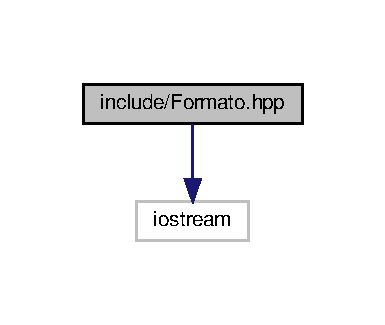
\includegraphics[width=185pt]{_formato_8hpp__incl}
\end{center}
\end{figure}
This graph shows which files directly or indirectly include this file\+:
\nopagebreak
\begin{figure}[H]
\begin{center}
\leavevmode
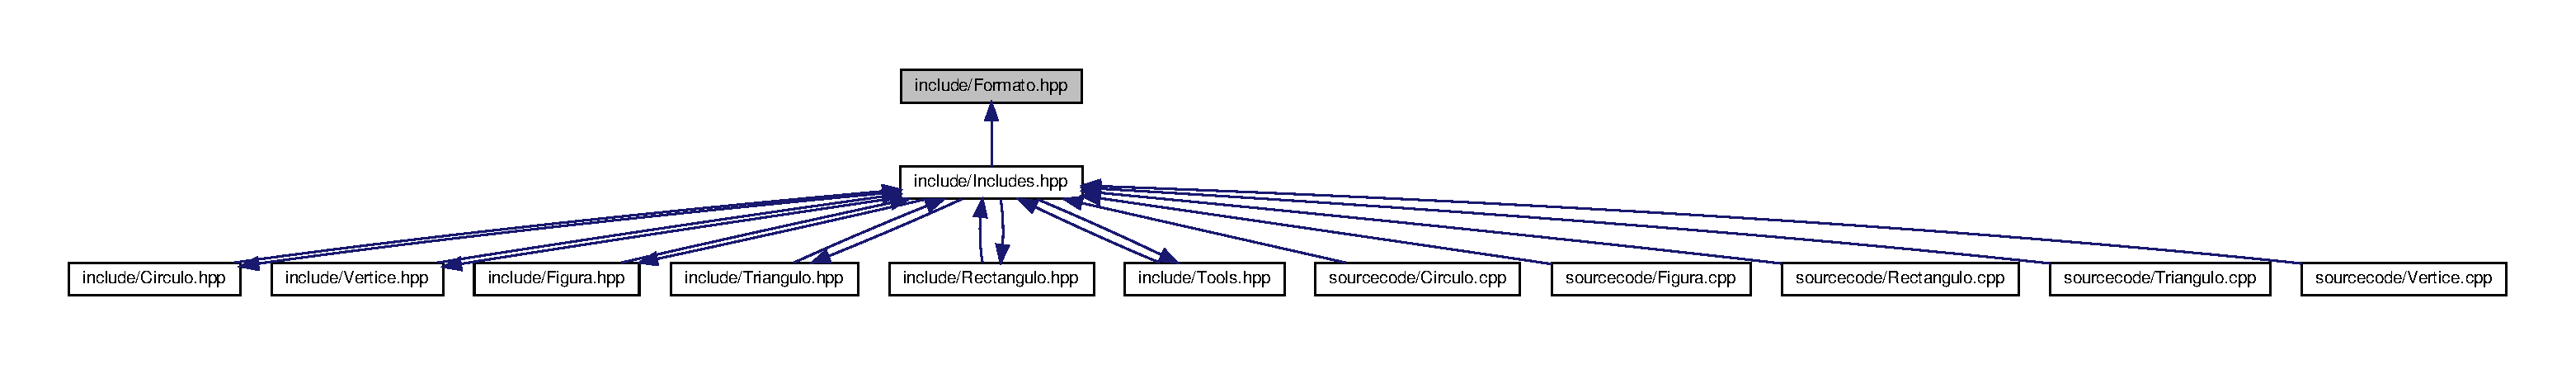
\includegraphics[width=350pt]{_formato_8hpp__dep__incl}
\end{center}
\end{figure}
\subsection*{Macros}
\begin{DoxyCompactItemize}
\item 
\mbox{\Hypertarget{_formato_8hpp_ae3b74adf57f76a62bd9fe44bb8d4695d}\label{_formato_8hpp_ae3b74adf57f76a62bd9fe44bb8d4695d}} 
\#define {\bfseries F\+O\+R\+M\+A\+T\+O\+\_\+\+A\+N\+S\+I\+\_\+\+C\+O\+L\+O\+R\+\_\+\+R\+E\+S\+ET}~\char`\"{}\textbackslash{}x1b\mbox{[}0m\char`\"{}
\item 
\mbox{\Hypertarget{_formato_8hpp_aed57c4d3731fc53122f7ee4bde3dde84}\label{_formato_8hpp_aed57c4d3731fc53122f7ee4bde3dde84}} 
\#define {\bfseries F\+O\+R\+M\+A\+T\+O\+\_\+\+A\+N\+S\+I\+\_\+\+C\+O\+L\+O\+R\+\_\+\+B\+L\+A\+CK}~\char`\"{}\textbackslash{}x1b\mbox{[}30m\char`\"{}
\item 
\mbox{\Hypertarget{_formato_8hpp_a3fedda2bfaffbadebe6c369c0d024c81}\label{_formato_8hpp_a3fedda2bfaffbadebe6c369c0d024c81}} 
\#define {\bfseries F\+O\+R\+M\+A\+T\+O\+\_\+\+A\+N\+S\+I\+\_\+\+C\+O\+L\+O\+R\+\_\+\+R\+ED}~\char`\"{}\textbackslash{}x1b\mbox{[}31m\char`\"{}
\item 
\mbox{\Hypertarget{_formato_8hpp_a30f3c6d0744f763c11c929dc58c7c442}\label{_formato_8hpp_a30f3c6d0744f763c11c929dc58c7c442}} 
\#define {\bfseries F\+O\+R\+M\+A\+T\+O\+\_\+\+A\+N\+S\+I\+\_\+\+C\+O\+L\+O\+R\+\_\+\+G\+R\+E\+EN}~\char`\"{}\textbackslash{}x1b\mbox{[}32m\char`\"{}
\item 
\mbox{\Hypertarget{_formato_8hpp_ac274e5edfd9450e72070bd9751f4d7a9}\label{_formato_8hpp_ac274e5edfd9450e72070bd9751f4d7a9}} 
\#define {\bfseries F\+O\+R\+M\+A\+T\+O\+\_\+\+A\+N\+S\+I\+\_\+\+C\+O\+L\+O\+R\+\_\+\+B\+R\+O\+WN}~\char`\"{}\textbackslash{}x1b\mbox{[}33m\char`\"{}
\item 
\mbox{\Hypertarget{_formato_8hpp_ad57e2554103db8b6cd12f58c33b36a68}\label{_formato_8hpp_ad57e2554103db8b6cd12f58c33b36a68}} 
\#define {\bfseries F\+O\+R\+M\+A\+T\+O\+\_\+\+A\+N\+S\+I\+\_\+\+C\+O\+L\+O\+R\+\_\+\+B\+L\+UE}~\char`\"{}\textbackslash{}x1b\mbox{[}34m\char`\"{}
\item 
\mbox{\Hypertarget{_formato_8hpp_a9be8ca01d2b905951cd9c18c0d4a8fbb}\label{_formato_8hpp_a9be8ca01d2b905951cd9c18c0d4a8fbb}} 
\#define {\bfseries F\+O\+R\+M\+A\+T\+O\+\_\+\+A\+N\+S\+I\+\_\+\+C\+O\+L\+O\+R\+\_\+\+P\+U\+R\+P\+LE}~\char`\"{}\textbackslash{}x1b\mbox{[}35m\char`\"{}
\item 
\mbox{\Hypertarget{_formato_8hpp_a1e6b735ded1de5f486c6bc768db19d4f}\label{_formato_8hpp_a1e6b735ded1de5f486c6bc768db19d4f}} 
\#define {\bfseries F\+O\+R\+M\+A\+T\+O\+\_\+\+A\+N\+S\+I\+\_\+\+C\+O\+L\+O\+R\+\_\+\+C\+Y\+AN}~\char`\"{}\textbackslash{}x1b\mbox{[}36m\char`\"{}
\item 
\mbox{\Hypertarget{_formato_8hpp_a2a90b61ed1404a9d6a1af268b37d3e56}\label{_formato_8hpp_a2a90b61ed1404a9d6a1af268b37d3e56}} 
\#define {\bfseries F\+O\+R\+M\+A\+T\+O\+\_\+\+A\+N\+S\+I\+\_\+\+C\+O\+L\+O\+R\+\_\+\+L\+I\+G\+T\+H\+\_\+\+G\+R\+AY}~\char`\"{}\textbackslash{}x1b\mbox{[}37m\char`\"{}
\item 
\mbox{\Hypertarget{_formato_8hpp_aeb975843c5f22d93a7a3cdef04c844e0}\label{_formato_8hpp_aeb975843c5f22d93a7a3cdef04c844e0}} 
\#define {\bfseries F\+O\+R\+M\+A\+T\+O\+\_\+\+A\+N\+S\+I\+\_\+\+C\+O\+L\+O\+R\+\_\+\+D\+A\+R\+K\+\_\+\+G\+R\+AY}~\char`\"{}\textbackslash{}x1b\mbox{[}01;30m\char`\"{}
\item 
\mbox{\Hypertarget{_formato_8hpp_ae79c129e8460c2eda3203f8ad81496a1}\label{_formato_8hpp_ae79c129e8460c2eda3203f8ad81496a1}} 
\#define {\bfseries F\+O\+R\+M\+A\+T\+O\+\_\+\+A\+N\+S\+I\+\_\+\+C\+O\+L\+O\+R\+\_\+\+L\+I\+G\+H\+T\+\_\+\+R\+ED}~\char`\"{}\textbackslash{}x1b\mbox{[}01;31m\char`\"{}
\item 
\mbox{\Hypertarget{_formato_8hpp_a3738c35591da00b0dd594b75df25c880}\label{_formato_8hpp_a3738c35591da00b0dd594b75df25c880}} 
\#define {\bfseries F\+O\+R\+M\+A\+T\+O\+\_\+\+A\+N\+S\+I\+\_\+\+C\+O\+L\+O\+R\+\_\+\+L\+I\+G\+H\+T\+\_\+\+G\+R\+E\+EN}~\char`\"{}\textbackslash{}x1b\mbox{[}01;32m\char`\"{}
\item 
\mbox{\Hypertarget{_formato_8hpp_a1134b02b205e250778fd55fb3bb4f7dd}\label{_formato_8hpp_a1134b02b205e250778fd55fb3bb4f7dd}} 
\#define {\bfseries F\+O\+R\+M\+A\+T\+O\+\_\+\+A\+N\+S\+I\+\_\+\+C\+O\+L\+O\+R\+\_\+\+Y\+E\+L\+L\+OW}~\char`\"{}\textbackslash{}x1b\mbox{[}01;33m\char`\"{}
\item 
\mbox{\Hypertarget{_formato_8hpp_a20ab1567abefed85bebe38d1f88f28ce}\label{_formato_8hpp_a20ab1567abefed85bebe38d1f88f28ce}} 
\#define {\bfseries F\+O\+R\+M\+A\+T\+O\+\_\+\+A\+N\+S\+I\+\_\+\+C\+O\+L\+O\+R\+\_\+\+L\+I\+G\+H\+T\+\_\+\+B\+L\+UE}~\char`\"{}\textbackslash{}x1b\mbox{[}01;34m\char`\"{}
\item 
\mbox{\Hypertarget{_formato_8hpp_a9b3ddb3e1c2dc61c19ff270563ba3faa}\label{_formato_8hpp_a9b3ddb3e1c2dc61c19ff270563ba3faa}} 
\#define {\bfseries F\+O\+R\+M\+A\+T\+O\+\_\+\+A\+N\+S\+I\+\_\+\+C\+O\+L\+O\+R\+\_\+\+L\+I\+G\+H\+T\+\_\+\+P\+U\+R\+P\+LE}~\char`\"{}\textbackslash{}x1b\mbox{[}01;35m\char`\"{}
\item 
\mbox{\Hypertarget{_formato_8hpp_aefe7241dd6f7d27f3585040073c72ddb}\label{_formato_8hpp_aefe7241dd6f7d27f3585040073c72ddb}} 
\#define {\bfseries F\+O\+R\+M\+A\+T\+O\+\_\+\+A\+N\+S\+I\+\_\+\+C\+O\+L\+O\+R\+\_\+\+L\+I\+G\+H\+T\+\_\+\+C\+Y\+AN}~\char`\"{}\textbackslash{}x1b\mbox{[}01;36m\char`\"{}
\item 
\mbox{\Hypertarget{_formato_8hpp_a4f58197deedea68acccd936af9e8b5be}\label{_formato_8hpp_a4f58197deedea68acccd936af9e8b5be}} 
\#define {\bfseries F\+O\+R\+M\+A\+T\+O\+\_\+\+A\+N\+S\+I\+\_\+\+C\+O\+L\+O\+R\+\_\+\+W\+H\+I\+TE}~\char`\"{}\textbackslash{}x1b\mbox{[}01;37m\char`\"{}
\item 
\mbox{\Hypertarget{_formato_8hpp_a7229d2fb244363c7e2f2e227a805171f}\label{_formato_8hpp_a7229d2fb244363c7e2f2e227a805171f}} 
\#define {\bfseries F\+O\+R\+M\+A\+T\+O\+\_\+\+B\+A\+C\+K\+G\+R\+O\+U\+N\+D\+\_\+\+C\+O\+L\+O\+R\+\_\+\+B\+L\+A\+CK}~\char`\"{}\textbackslash{}x1b\mbox{[}40m\char`\"{}
\item 
\mbox{\Hypertarget{_formato_8hpp_a079f709bdab88dc8ff2978cac78a866c}\label{_formato_8hpp_a079f709bdab88dc8ff2978cac78a866c}} 
\#define {\bfseries F\+O\+R\+M\+A\+T\+O\+\_\+\+B\+A\+C\+K\+G\+R\+O\+U\+N\+D\+\_\+\+C\+O\+L\+O\+R\+\_\+\+R\+ED}~\char`\"{}\textbackslash{}x1b\mbox{[}41m\char`\"{}
\item 
\mbox{\Hypertarget{_formato_8hpp_af02eb9759922a233cd781ec3dbe2c746}\label{_formato_8hpp_af02eb9759922a233cd781ec3dbe2c746}} 
\#define {\bfseries F\+O\+R\+M\+A\+T\+O\+\_\+\+B\+A\+C\+K\+G\+R\+O\+U\+N\+D\+\_\+\+C\+O\+L\+O\+R\+\_\+\+G\+R\+E\+EN}~\char`\"{}\textbackslash{}x1b\mbox{[}42m\char`\"{}
\item 
\mbox{\Hypertarget{_formato_8hpp_afce78df9fb502edfc071f5307acf7484}\label{_formato_8hpp_afce78df9fb502edfc071f5307acf7484}} 
\#define {\bfseries F\+O\+R\+M\+A\+T\+O\+\_\+\+B\+A\+C\+K\+G\+R\+O\+U\+N\+D\+\_\+\+C\+O\+L\+O\+R\+\_\+\+B\+R\+O\+WN}~\char`\"{}\textbackslash{}x1b\mbox{[}43m\char`\"{}
\item 
\mbox{\Hypertarget{_formato_8hpp_a8cc645fa686dfc85d7a2136065f97490}\label{_formato_8hpp_a8cc645fa686dfc85d7a2136065f97490}} 
\#define {\bfseries F\+O\+R\+M\+A\+T\+O\+\_\+\+B\+A\+C\+K\+G\+R\+O\+U\+N\+D\+\_\+\+C\+O\+L\+O\+R\+\_\+\+B\+L\+UE}~\char`\"{}\textbackslash{}x1b\mbox{[}44m\char`\"{}
\item 
\mbox{\Hypertarget{_formato_8hpp_a0640c3a1cc415872af00083acf1f92c7}\label{_formato_8hpp_a0640c3a1cc415872af00083acf1f92c7}} 
\#define {\bfseries F\+O\+R\+M\+A\+T\+O\+\_\+\+B\+A\+C\+K\+G\+R\+O\+U\+N\+D\+\_\+\+C\+O\+L\+O\+R\+\_\+\+P\+U\+R\+P\+LE}~\char`\"{}\textbackslash{}x1b\mbox{[}45m\char`\"{}
\item 
\mbox{\Hypertarget{_formato_8hpp_a6ffb7f0c33ea0dd799613da7c906437c}\label{_formato_8hpp_a6ffb7f0c33ea0dd799613da7c906437c}} 
\#define {\bfseries F\+O\+R\+M\+A\+T\+O\+\_\+\+B\+A\+C\+K\+G\+R\+O\+U\+N\+D\+\_\+\+C\+O\+L\+O\+R\+\_\+\+T\+U\+R\+Q\+U\+O\+I\+SE}~\char`\"{}\textbackslash{}x1b\mbox{[}46m\char`\"{}
\item 
\mbox{\Hypertarget{_formato_8hpp_addf0aca1b7807ccf9046a00d6273111a}\label{_formato_8hpp_addf0aca1b7807ccf9046a00d6273111a}} 
\#define {\bfseries F\+O\+R\+M\+A\+T\+O\+\_\+\+B\+A\+C\+K\+G\+R\+O\+U\+N\+D\+\_\+\+C\+O\+L\+O\+R\+\_\+\+G\+R\+AY}~\char`\"{}\textbackslash{}x1b\mbox{[}40m\char`\"{}
\item 
\mbox{\Hypertarget{_formato_8hpp_a41f1b9682dda71d9d21d5fbadc36e85a}\label{_formato_8hpp_a41f1b9682dda71d9d21d5fbadc36e85a}} 
\#define {\bfseries F\+O\+R\+M\+A\+T\+O\+\_\+\+B\+A\+C\+K\+G\+R\+O\+U\+N\+D\+\_\+\+C\+O\+L\+O\+R\+\_\+\+D\+A\+R\+K\+\_\+\+G\+R\+AY}~\char`\"{}\textbackslash{}x1b\mbox{[}100m\char`\"{}
\item 
\mbox{\Hypertarget{_formato_8hpp_ab942fb55df7112f64400cd95d2433fc2}\label{_formato_8hpp_ab942fb55df7112f64400cd95d2433fc2}} 
\#define {\bfseries F\+O\+R\+M\+A\+T\+O\+\_\+\+B\+A\+C\+K\+G\+R\+O\+U\+N\+D\+\_\+\+C\+O\+L\+O\+R\+\_\+\+L\+I\+G\+T\+H\+\_\+\+R\+ED}~\char`\"{}\textbackslash{}x1b\mbox{[}101m\char`\"{}
\item 
\mbox{\Hypertarget{_formato_8hpp_adff2cf72fd266a80140877b69f14935c}\label{_formato_8hpp_adff2cf72fd266a80140877b69f14935c}} 
\#define {\bfseries F\+O\+R\+M\+A\+T\+O\+\_\+\+B\+A\+C\+K\+G\+R\+O\+U\+N\+D\+\_\+\+C\+O\+L\+O\+R\+\_\+\+L\+I\+G\+T\+H\+\_\+\+G\+R\+E\+EN}~\char`\"{}\textbackslash{}x1b\mbox{[}102m\char`\"{}
\item 
\mbox{\Hypertarget{_formato_8hpp_afab9dc04e19502c5246cadfb14b10810}\label{_formato_8hpp_afab9dc04e19502c5246cadfb14b10810}} 
\#define {\bfseries F\+O\+R\+M\+A\+T\+O\+\_\+\+B\+A\+C\+K\+G\+R\+O\+U\+N\+D\+\_\+\+C\+O\+L\+O\+R\+\_\+\+L\+I\+G\+T\+H\+\_\+\+Y\+E\+L\+L\+OW}~\char`\"{}\textbackslash{}x1b\mbox{[}103m\char`\"{}
\item 
\mbox{\Hypertarget{_formato_8hpp_a2b7330f580c322bc6a2120c26b3c3ef0}\label{_formato_8hpp_a2b7330f580c322bc6a2120c26b3c3ef0}} 
\#define {\bfseries F\+O\+R\+M\+A\+T\+O\+\_\+\+B\+A\+C\+K\+G\+R\+O\+U\+N\+D\+\_\+\+C\+O\+L\+O\+R\+\_\+\+L\+I\+G\+T\+H\+\_\+\+B\+L\+UE}~\char`\"{}\textbackslash{}x1b\mbox{[}104m\char`\"{}
\item 
\mbox{\Hypertarget{_formato_8hpp_a50f2c55f3674afcd613b54c6ce792b73}\label{_formato_8hpp_a50f2c55f3674afcd613b54c6ce792b73}} 
\#define {\bfseries F\+O\+R\+M\+A\+T\+O\+\_\+\+B\+A\+C\+K\+G\+R\+O\+U\+N\+D\+\_\+\+C\+O\+L\+O\+R\+\_\+\+L\+I\+G\+T\+H\+\_\+\+P\+U\+R\+P\+LE}~\char`\"{}\textbackslash{}x1b\mbox{[}105m\char`\"{}
\item 
\mbox{\Hypertarget{_formato_8hpp_a7f9d2ab548110b3195d2f7cc7ea71f0c}\label{_formato_8hpp_a7f9d2ab548110b3195d2f7cc7ea71f0c}} 
\#define {\bfseries F\+O\+R\+M\+A\+T\+O\+\_\+\+B\+A\+C\+K\+G\+R\+O\+U\+N\+D\+\_\+\+C\+O\+L\+O\+R\+\_\+\+L\+I\+G\+T\+H\+\_\+\+T\+U\+R\+Q\+U\+O\+I\+SE}~\char`\"{}\textbackslash{}x1b\mbox{[}106m\char`\"{}
\item 
\mbox{\Hypertarget{_formato_8hpp_ad617c31e7833166f7bbec8172b90974a}\label{_formato_8hpp_ad617c31e7833166f7bbec8172b90974a}} 
\#define {\bfseries F\+O\+R\+M\+A\+T\+O\+\_\+\+B\+A\+C\+K\+G\+R\+O\+U\+N\+D\+\_\+\+C\+O\+L\+O\+R\+\_\+\+W\+H\+I\+TE}~\char`\"{}\textbackslash{}x1b\mbox{[}107m\char`\"{}
\item 
\mbox{\Hypertarget{_formato_8hpp_a030402feca49920979ca10fb2e00663b}\label{_formato_8hpp_a030402feca49920979ca10fb2e00663b}} 
\#define {\bfseries F\+O\+R\+M\+A\+T\+O\+\_\+\+U\+N\+D\+E\+R\+L\+I\+N\+E\+\_\+\+E\+F\+F\+E\+CT}~\char`\"{}\textbackslash{}x1b\mbox{[}00;4m\char`\"{}
\item 
\mbox{\Hypertarget{_formato_8hpp_aebb3b68dbe39833a4b08a42ff9e903bb}\label{_formato_8hpp_aebb3b68dbe39833a4b08a42ff9e903bb}} 
\#define {\bfseries F\+O\+R\+M\+A\+T\+O\+\_\+\+B\+L\+I\+N\+K\+\_\+\+E\+F\+F\+E\+CT}~\char`\"{}\textbackslash{}x1b\mbox{[}00;5m\char`\"{}
\item 
\mbox{\Hypertarget{_formato_8hpp_a944683098049f3c505f95ad0c39bf136}\label{_formato_8hpp_a944683098049f3c505f95ad0c39bf136}} 
\#define {\bfseries F\+O\+R\+M\+A\+T\+O\+\_\+\+B\+O\+L\+D\+\_\+\+E\+F\+F\+E\+CT}~\char`\"{}\textbackslash{}x1b\mbox{[}00;1m\char`\"{}
\item 
\mbox{\Hypertarget{_formato_8hpp_a1ddbe280314bf3ba383fd6940860d957}\label{_formato_8hpp_a1ddbe280314bf3ba383fd6940860d957}} 
\#define {\bfseries F\+O\+R\+M\+A\+T\+O\+\_\+\+T\+R\+A\+N\+S\+P\+A\+R\+E\+N\+T\+\_\+\+E\+F\+F\+E\+CT}~\char`\"{}\textbackslash{}x1b\mbox{[}00;8m\char`\"{}
\end{DoxyCompactItemize}


\subsection{Detailed Description}
/ 
\hypertarget{_impresora_8hpp}{}\section{include/\+Impresora.hpp File Reference}
\label{_impresora_8hpp}\index{include/\+Impresora.\+hpp@{include/\+Impresora.\+hpp}}
This graph shows which files directly or indirectly include this file\+:
\nopagebreak
\begin{figure}[H]
\begin{center}
\leavevmode
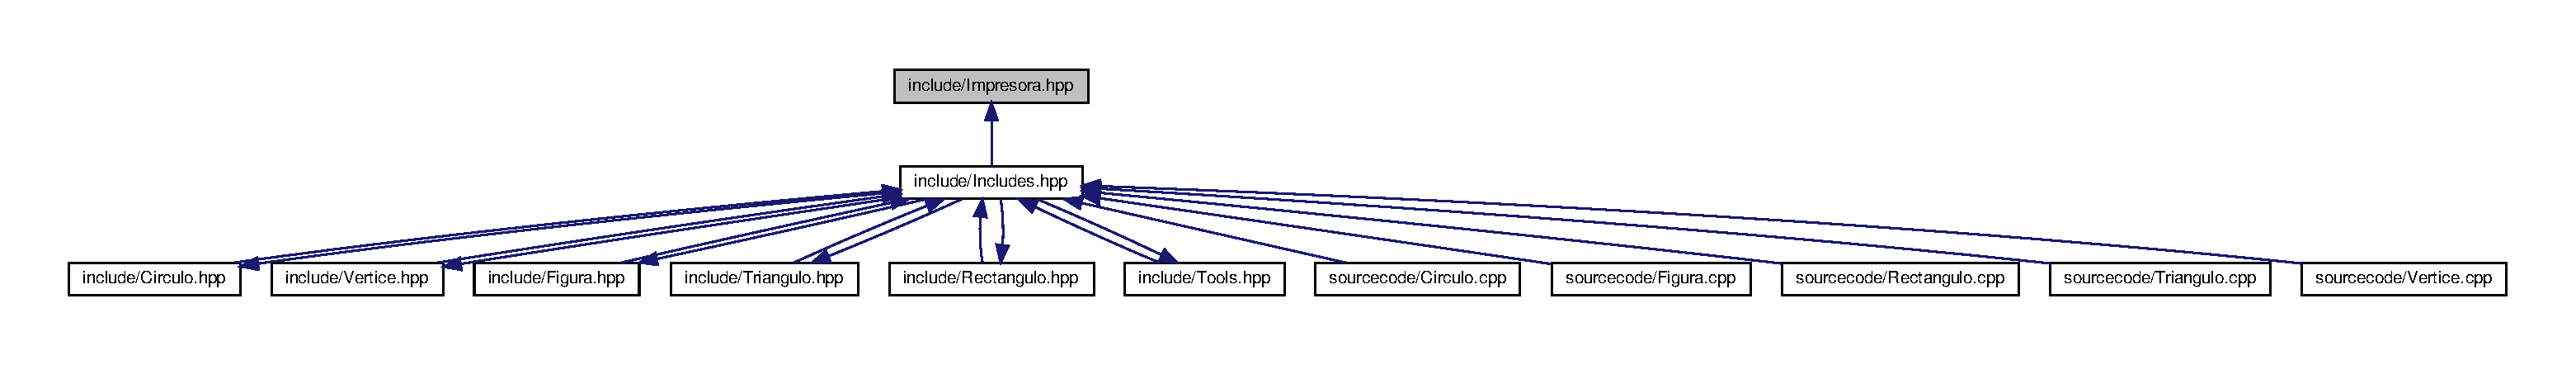
\includegraphics[width=350pt]{_impresora_8hpp__dep__incl}
\end{center}
\end{figure}
\subsection*{Classes}
\begin{DoxyCompactItemize}
\item 
class \hyperlink{class_impresora}{Impresora$<$ T $>$}
\begin{DoxyCompactList}\small\item\em clase que imprmime objetos \end{DoxyCompactList}\end{DoxyCompactItemize}


\subsection{Detailed Description}
/ 
\hypertarget{_includes_8hpp}{}\section{include/\+Includes.hpp File Reference}
\label{_includes_8hpp}\index{include/\+Includes.\+hpp@{include/\+Includes.\+hpp}}
{\ttfamily \#include $<$opencv2/highgui.\+hpp$>$}\newline
{\ttfamily \#include $<$opencv/cv.\+hpp$>$}\newline
{\ttfamily \#include $<$iostream$>$}\newline
{\ttfamily \#include $<$stdlib.\+h$>$}\newline
{\ttfamily \#include $<$chrono$>$}\newline
{\ttfamily \#include $<$random$>$}\newline
{\ttfamily \#include $<$fstream$>$}\newline
{\ttfamily \#include $<$math.\+h$>$}\newline
{\ttfamily \#include $<$cmath$>$}\newline
{\ttfamily \#include \char`\"{}./\+Filtros.\+hpp\char`\"{}}\newline
{\ttfamily \#include $<$Magick++.\+h$>$}\newline
Include dependency graph for Includes.\+hpp\+:
\nopagebreak
\begin{figure}[H]
\begin{center}
\leavevmode
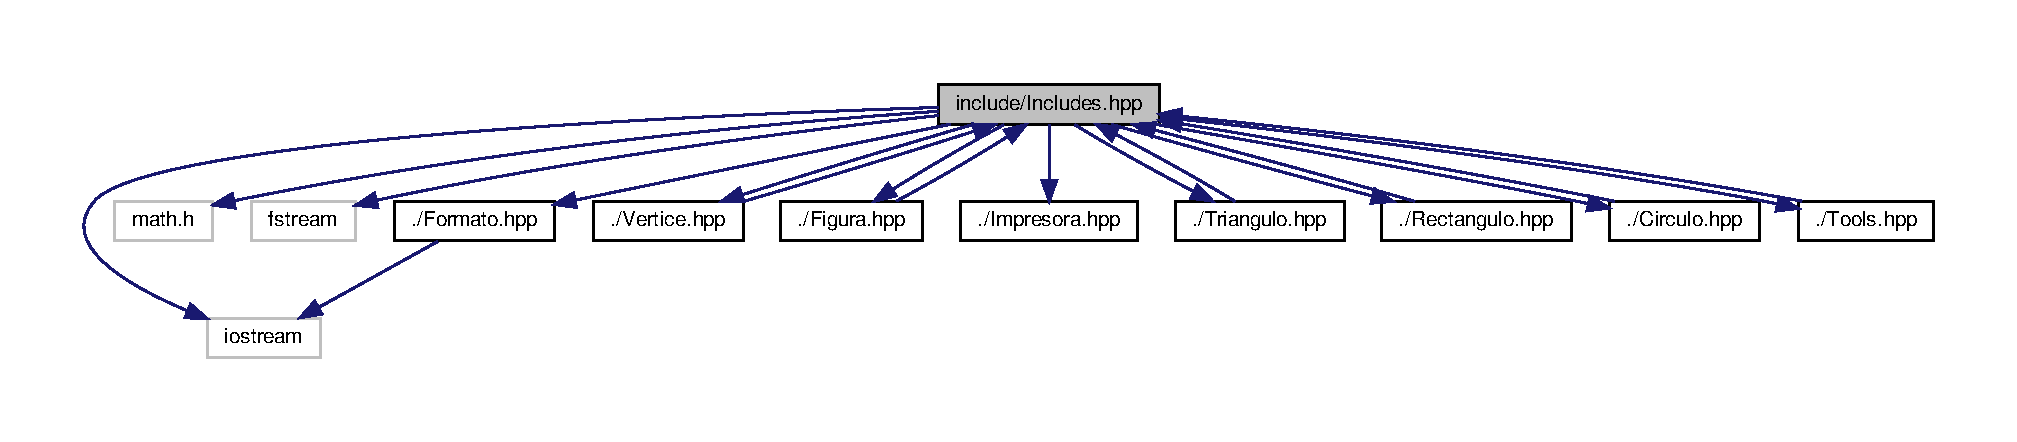
\includegraphics[width=350pt]{_includes_8hpp__incl}
\end{center}
\end{figure}
This graph shows which files directly or indirectly include this file\+:
\nopagebreak
\begin{figure}[H]
\begin{center}
\leavevmode
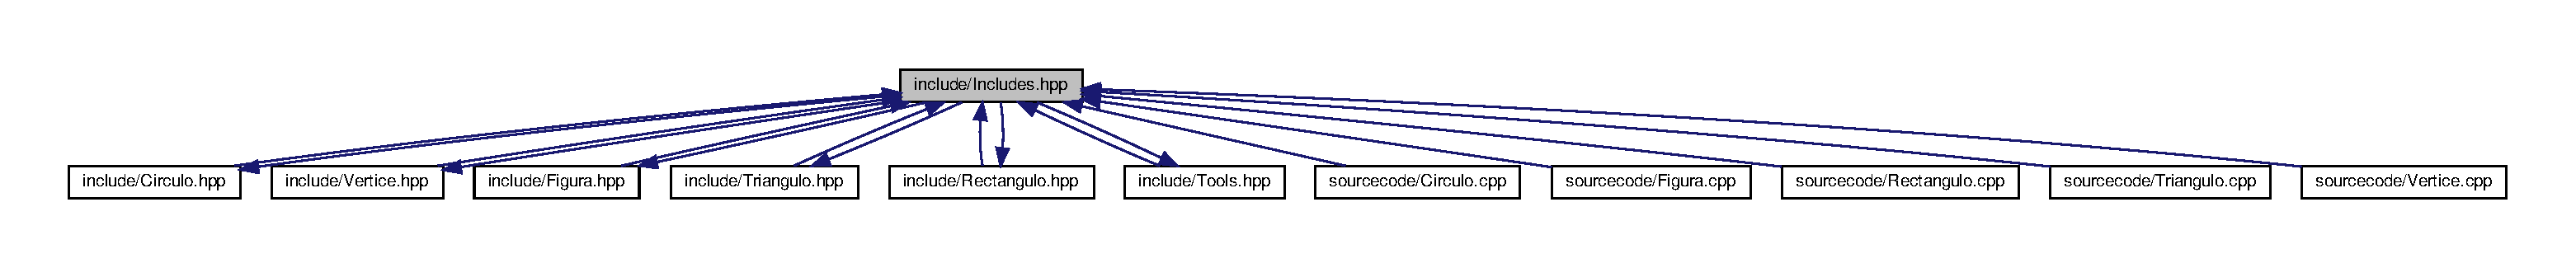
\includegraphics[width=350pt]{_includes_8hpp__dep__incl}
\end{center}
\end{figure}


\subsection{Detailed Description}
/ 
\hypertarget{_rectangulo_8hpp}{}\section{include/\+Rectangulo.hpp File Reference}
\label{_rectangulo_8hpp}\index{include/\+Rectangulo.\+hpp@{include/\+Rectangulo.\+hpp}}
{\ttfamily \#include \char`\"{}./\+Includes.\+hpp\char`\"{}}\newline
Include dependency graph for Rectangulo.\+hpp\+:
\nopagebreak
\begin{figure}[H]
\begin{center}
\leavevmode
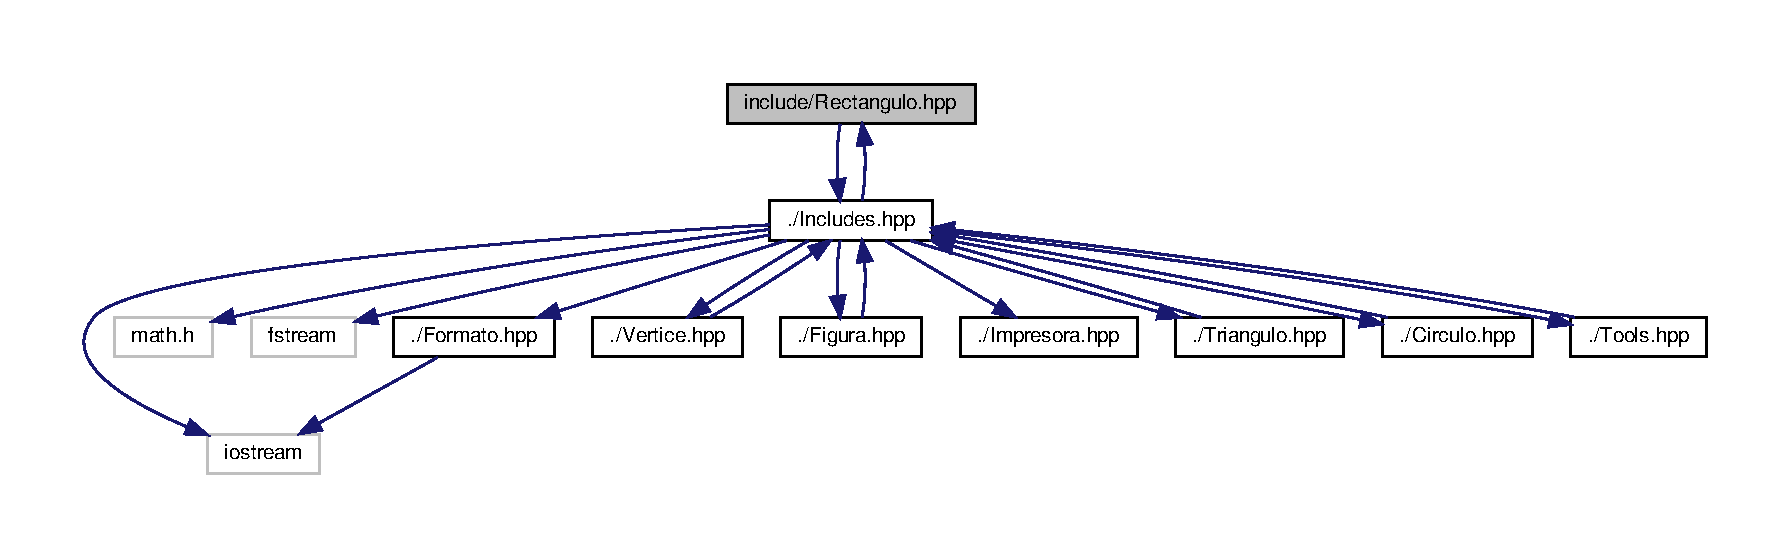
\includegraphics[width=350pt]{_rectangulo_8hpp__incl}
\end{center}
\end{figure}
This graph shows which files directly or indirectly include this file\+:
\nopagebreak
\begin{figure}[H]
\begin{center}
\leavevmode
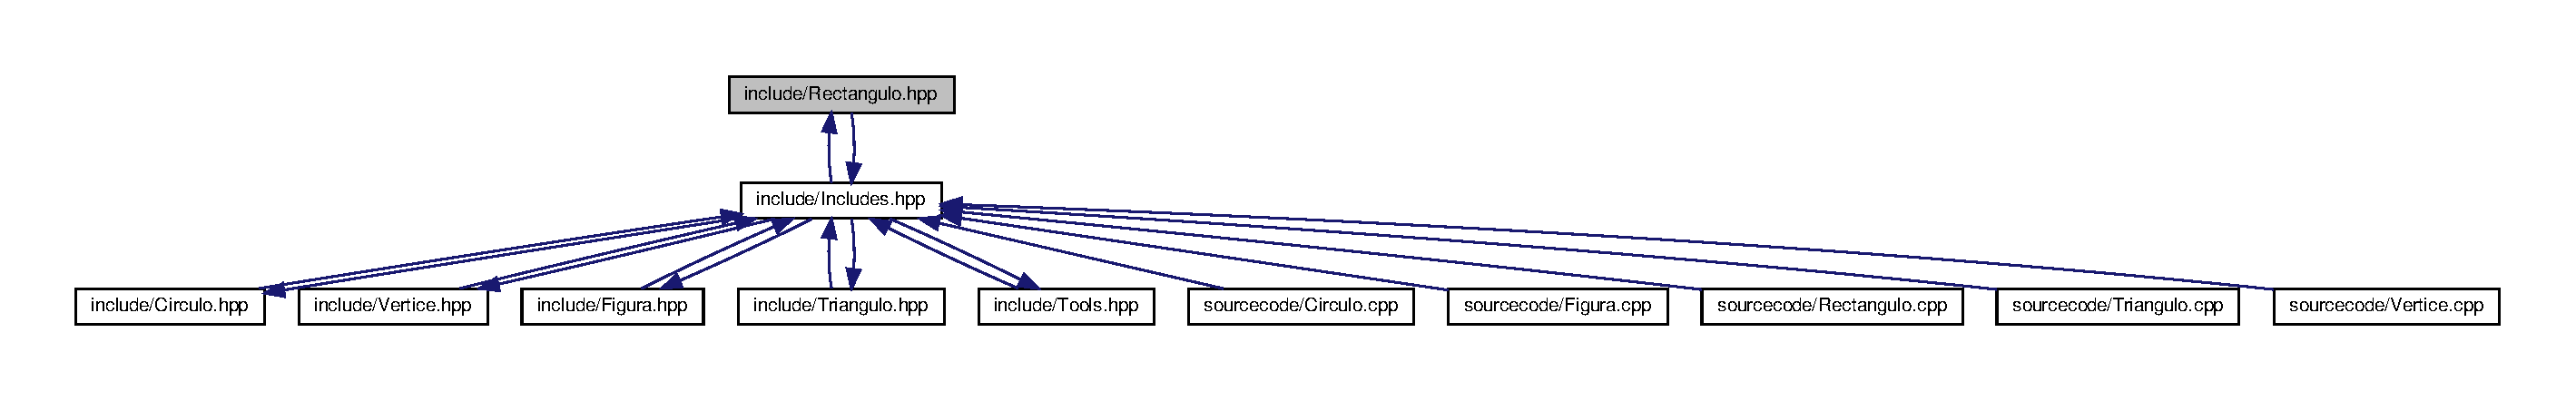
\includegraphics[width=350pt]{_rectangulo_8hpp__dep__incl}
\end{center}
\end{figure}
\subsection*{Classes}
\begin{DoxyCompactItemize}
\item 
class \hyperlink{classrectangulo}{rectangulo}
\begin{DoxyCompactList}\small\item\em Clase rectangulo. \end{DoxyCompactList}\end{DoxyCompactItemize}


\subsection{Detailed Description}
/ 
\hypertarget{_tools_8hpp}{}\section{include/\+Tools.hpp File Reference}
\label{_tools_8hpp}\index{include/\+Tools.\+hpp@{include/\+Tools.\+hpp}}
{\ttfamily \#include \char`\"{}./\+Includes.\+hpp\char`\"{}}\newline
Include dependency graph for Tools.\+hpp\+:
\nopagebreak
\begin{figure}[H]
\begin{center}
\leavevmode
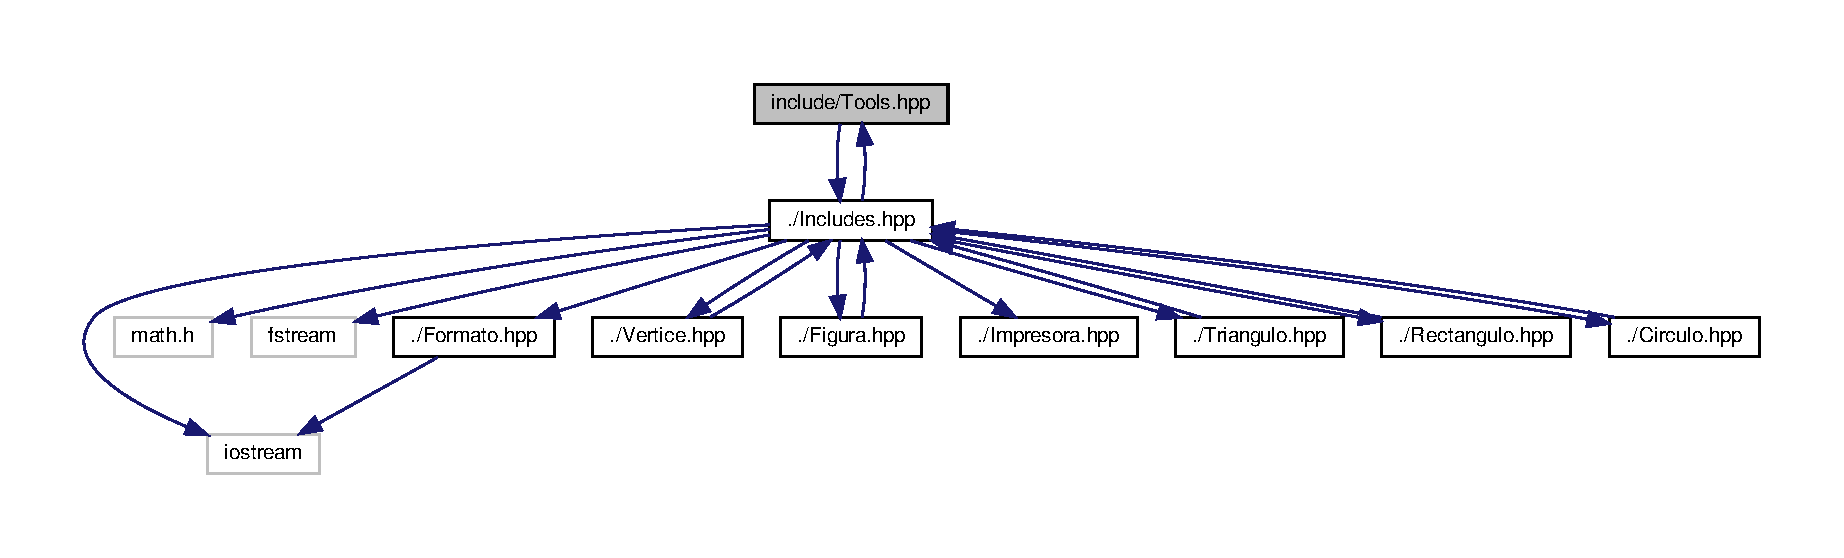
\includegraphics[width=350pt]{_tools_8hpp__incl}
\end{center}
\end{figure}
This graph shows which files directly or indirectly include this file\+:
\nopagebreak
\begin{figure}[H]
\begin{center}
\leavevmode
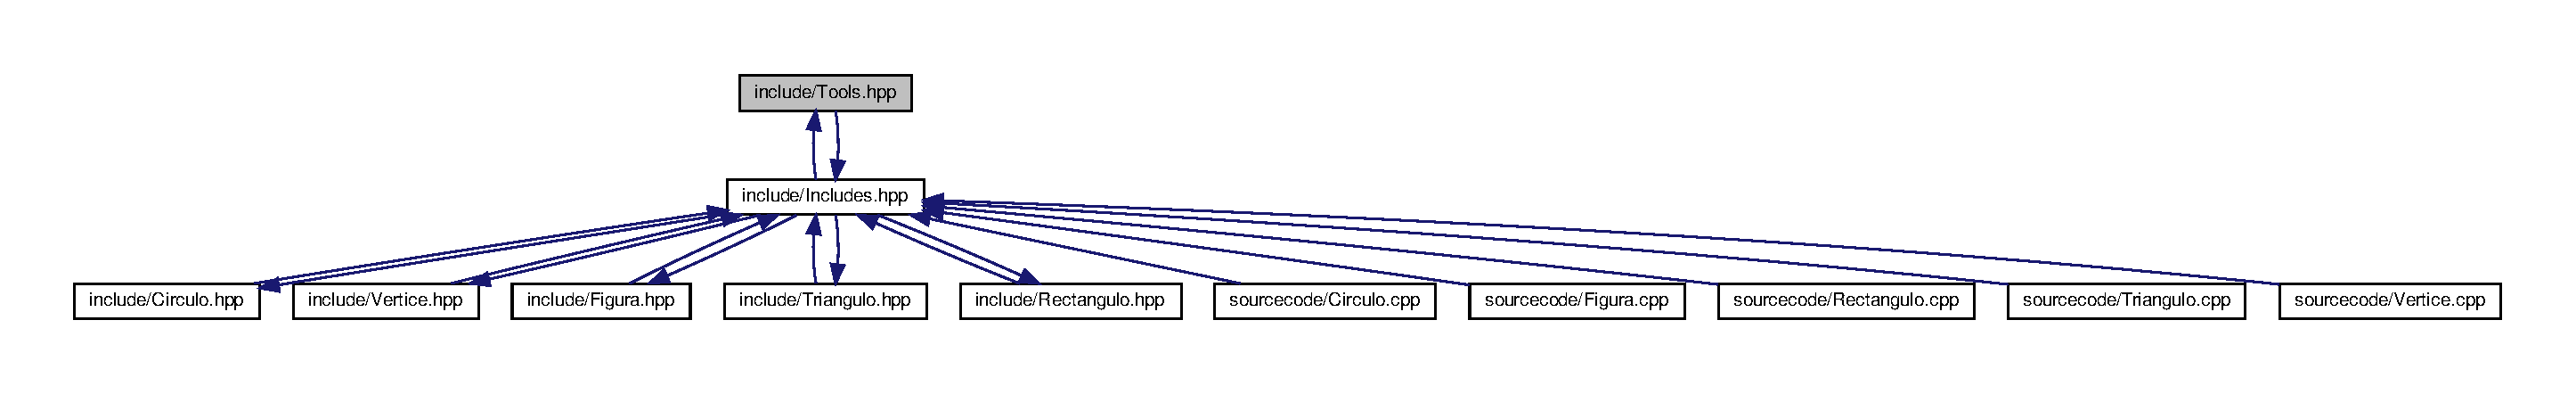
\includegraphics[width=350pt]{_tools_8hpp__dep__incl}
\end{center}
\end{figure}
\subsection*{Classes}
\begin{DoxyCompactItemize}
\item 
class \hyperlink{class_principal}{Principal}
\end{DoxyCompactItemize}


\subsection{Detailed Description}
/ 
\hypertarget{_triangulo_8hpp}{}\section{include/\+Triangulo.hpp File Reference}
\label{_triangulo_8hpp}\index{include/\+Triangulo.\+hpp@{include/\+Triangulo.\+hpp}}
{\ttfamily \#include \char`\"{}./\+Includes.\+hpp\char`\"{}}\newline
Include dependency graph for Triangulo.\+hpp\+:
\nopagebreak
\begin{figure}[H]
\begin{center}
\leavevmode
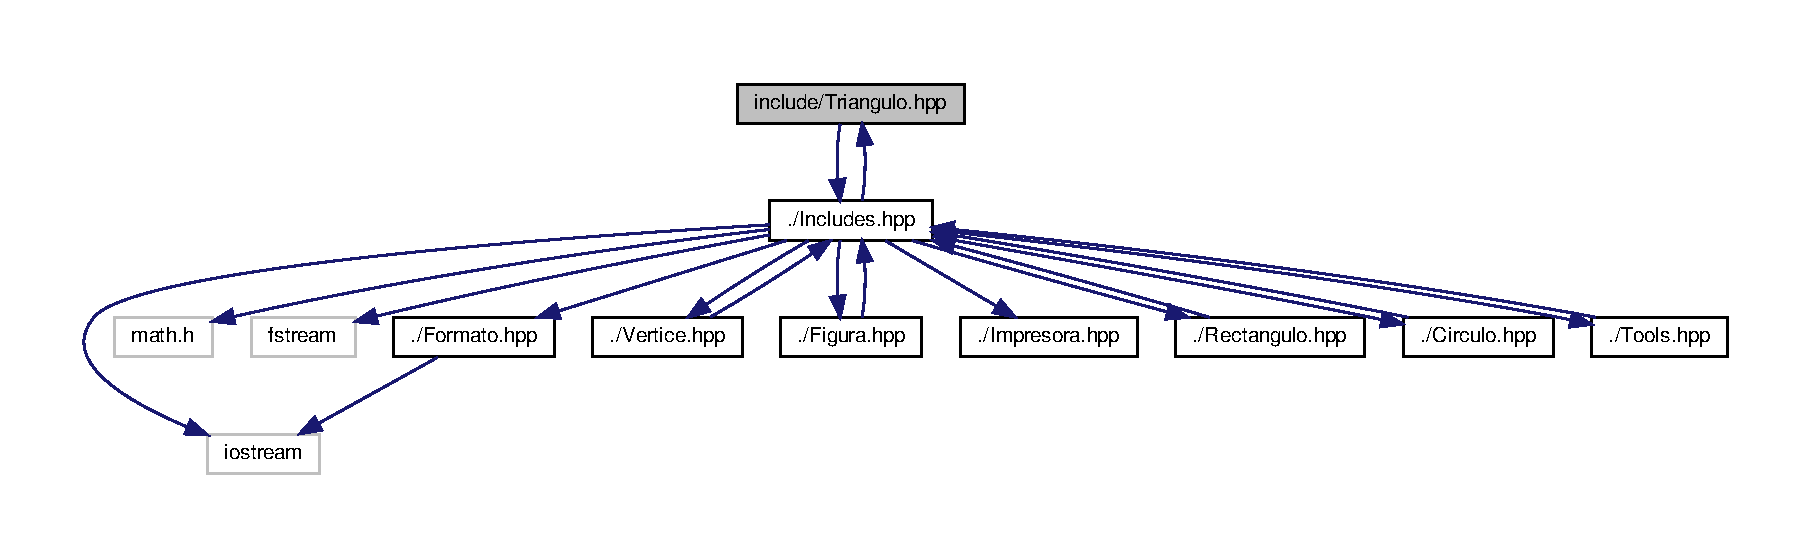
\includegraphics[width=350pt]{_triangulo_8hpp__incl}
\end{center}
\end{figure}
This graph shows which files directly or indirectly include this file\+:
\nopagebreak
\begin{figure}[H]
\begin{center}
\leavevmode
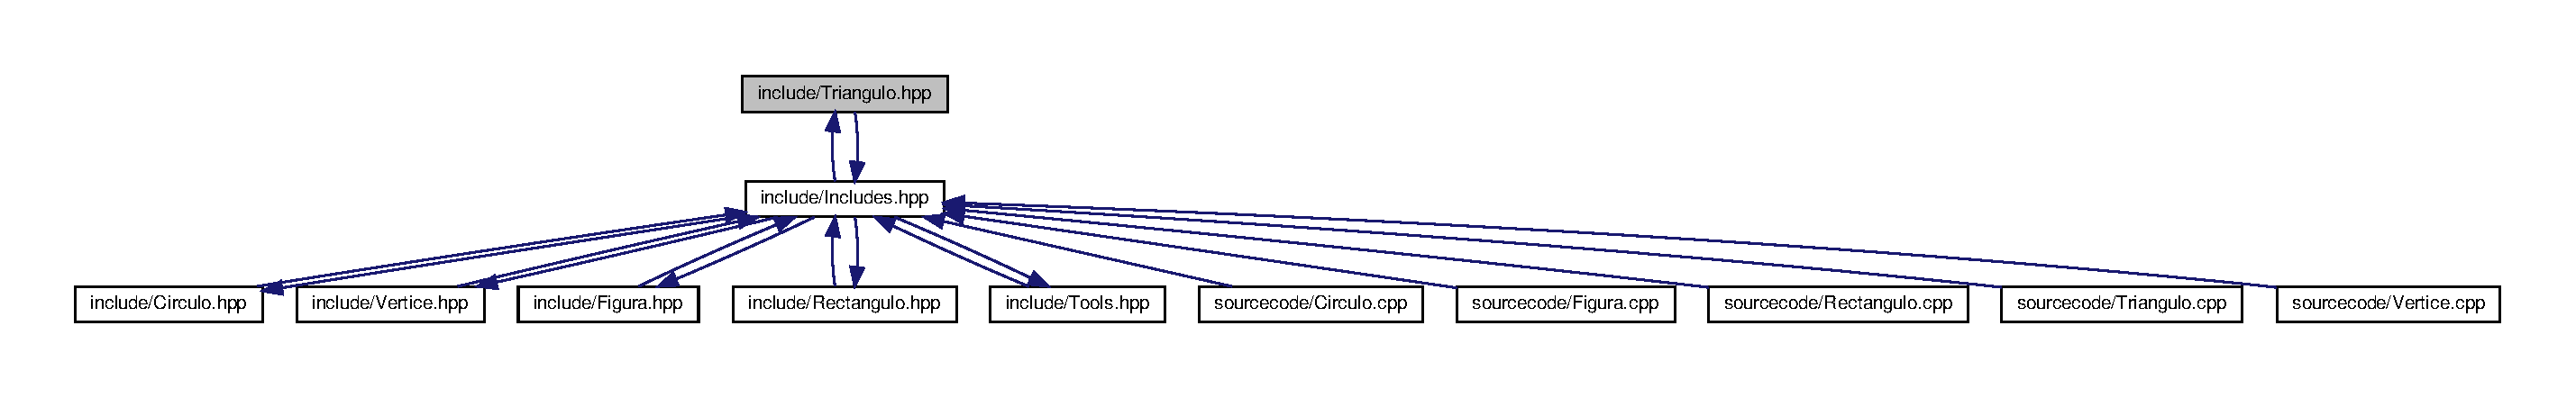
\includegraphics[width=350pt]{_triangulo_8hpp__dep__incl}
\end{center}
\end{figure}
\subsection*{Classes}
\begin{DoxyCompactItemize}
\item 
class \hyperlink{classtriangulo}{triangulo}
\begin{DoxyCompactList}\small\item\em calse tringulo \end{DoxyCompactList}\item 
class \hyperlink{class_escaleno}{Escaleno}
\begin{DoxyCompactList}\small\item\em calse \hyperlink{class_escaleno}{Escaleno} \end{DoxyCompactList}\item 
class \hyperlink{class_equilatero}{Equilatero}
\begin{DoxyCompactList}\small\item\em calse equilatero \end{DoxyCompactList}\item 
class \hyperlink{class_isosceles}{Isosceles}
\begin{DoxyCompactList}\small\item\em calse \hyperlink{class_isosceles}{Isosceles} \end{DoxyCompactList}\end{DoxyCompactItemize}


\subsection{Detailed Description}
/ 
\hypertarget{_vertice_8hpp}{}\section{include/\+Vertice.hpp File Reference}
\label{_vertice_8hpp}\index{include/\+Vertice.\+hpp@{include/\+Vertice.\+hpp}}
{\ttfamily \#include \char`\"{}./\+Includes.\+hpp\char`\"{}}\newline
Include dependency graph for Vertice.\+hpp\+:
\nopagebreak
\begin{figure}[H]
\begin{center}
\leavevmode
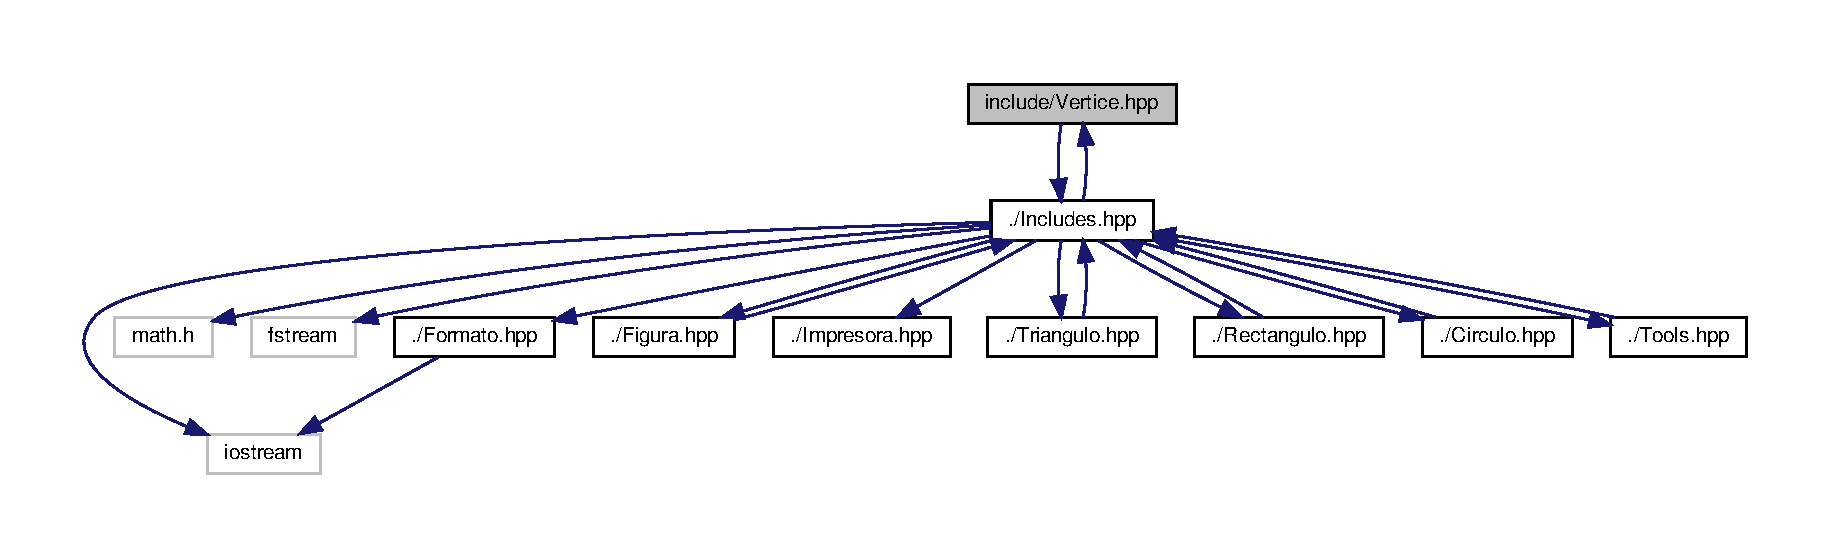
\includegraphics[width=350pt]{_vertice_8hpp__incl}
\end{center}
\end{figure}
This graph shows which files directly or indirectly include this file\+:
\nopagebreak
\begin{figure}[H]
\begin{center}
\leavevmode
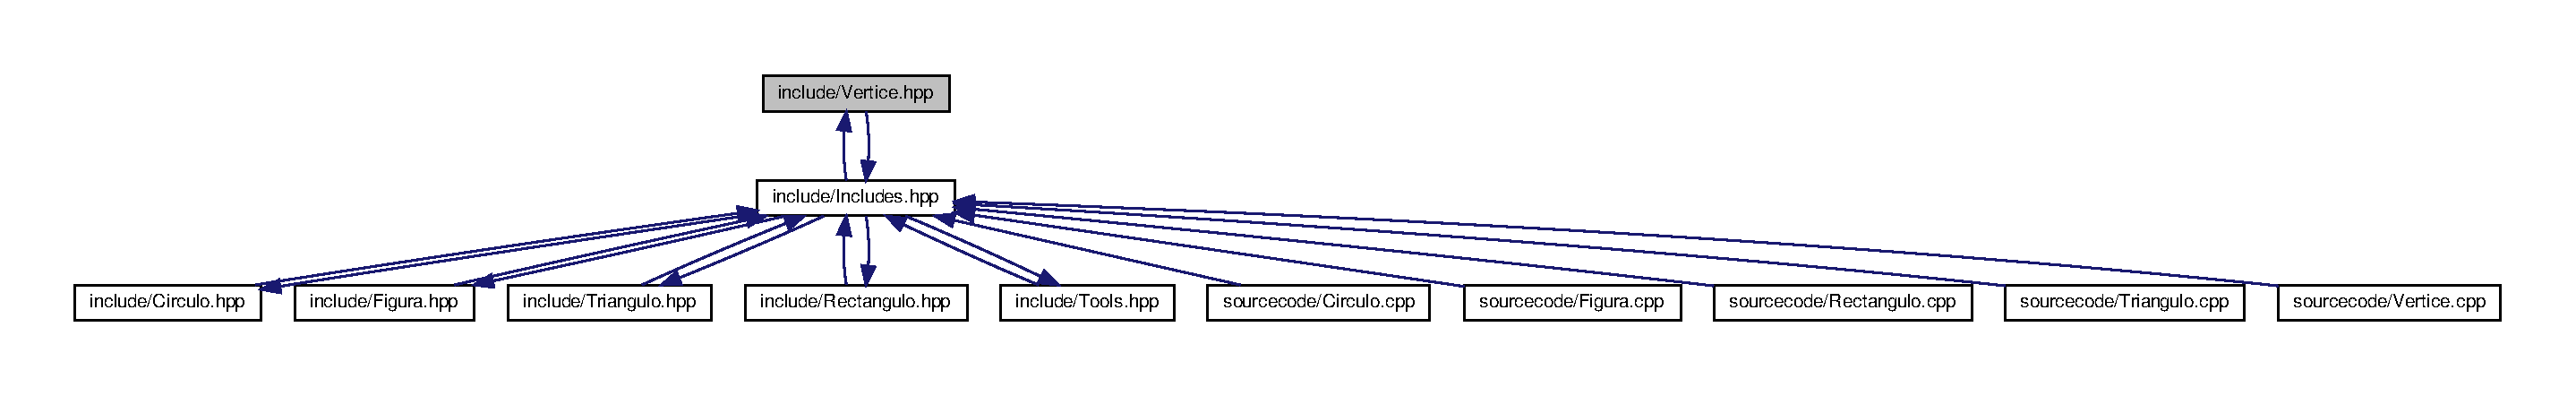
\includegraphics[width=350pt]{_vertice_8hpp__dep__incl}
\end{center}
\end{figure}
\subsection*{Classes}
\begin{DoxyCompactItemize}
\item 
class \hyperlink{class_vertice}{Vertice}
\begin{DoxyCompactList}\small\item\em clase que modela un punto en el espacio \end{DoxyCompactList}\end{DoxyCompactItemize}


\subsection{Detailed Description}
/ 
\hypertarget{_circulo_8cpp}{}\section{sourcecode/\+Circulo.cpp File Reference}
\label{_circulo_8cpp}\index{sourcecode/\+Circulo.\+cpp@{sourcecode/\+Circulo.\+cpp}}
{\ttfamily \#include \char`\"{}../include/\+Includes.\+hpp\char`\"{}}\newline
Include dependency graph for Circulo.\+cpp\+:
\nopagebreak
\begin{figure}[H]
\begin{center}
\leavevmode
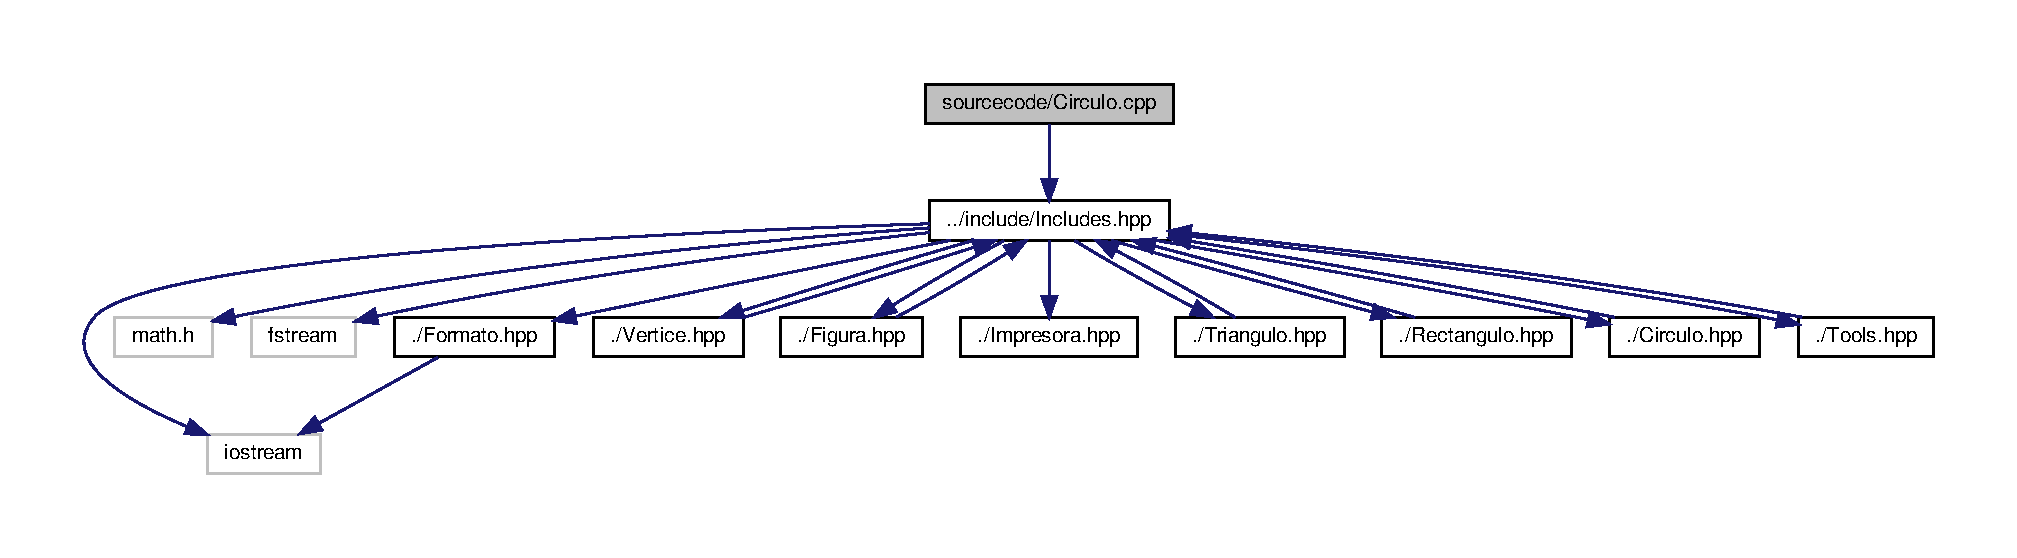
\includegraphics[width=350pt]{_circulo_8cpp__incl}
\end{center}
\end{figure}


\subsection{Detailed Description}
/ 
\hypertarget{_figura_8cpp}{}\section{sourcecode/\+Figura.cpp File Reference}
\label{_figura_8cpp}\index{sourcecode/\+Figura.\+cpp@{sourcecode/\+Figura.\+cpp}}
{\ttfamily \#include \char`\"{}../include/\+Includes.\+hpp\char`\"{}}\newline
Include dependency graph for Figura.\+cpp\+:
\nopagebreak
\begin{figure}[H]
\begin{center}
\leavevmode
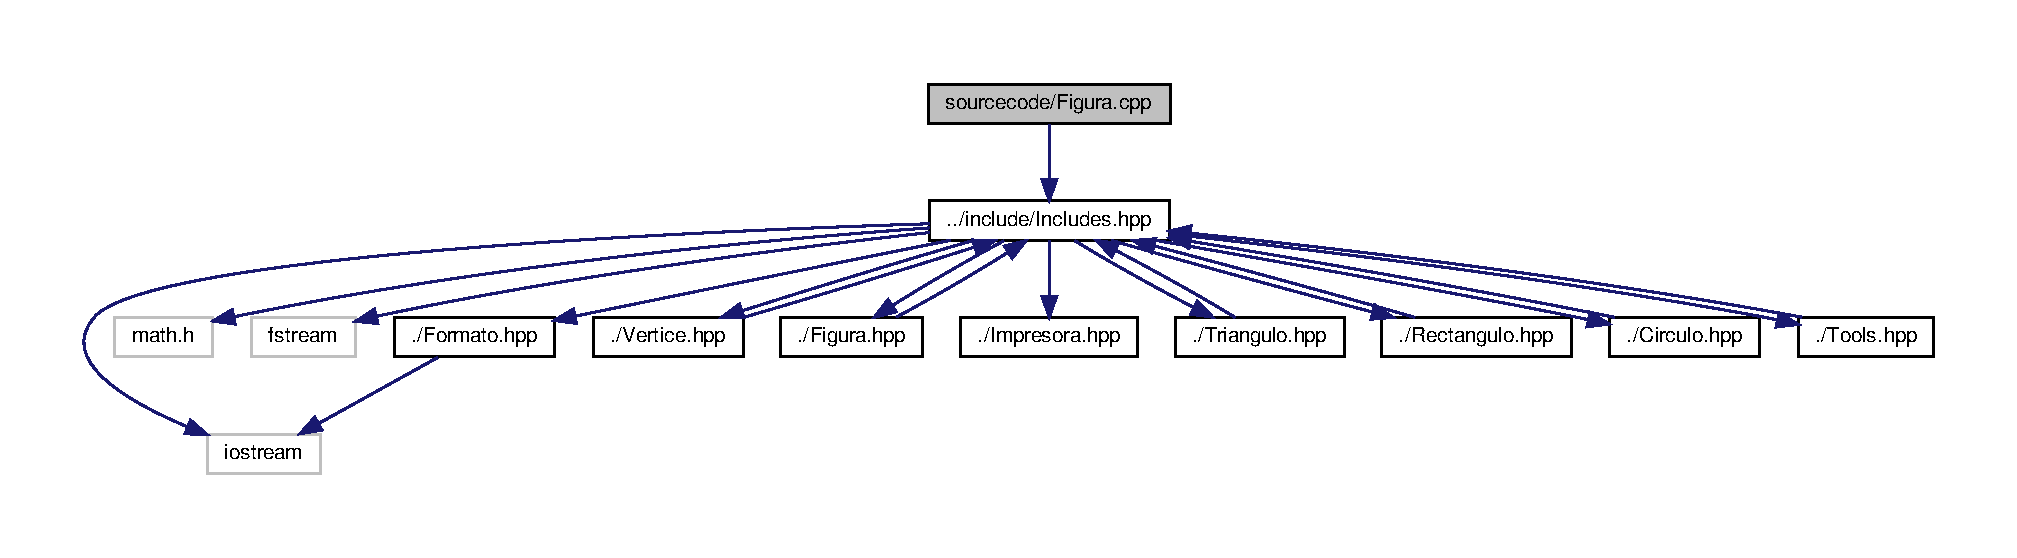
\includegraphics[width=350pt]{_figura_8cpp__incl}
\end{center}
\end{figure}


\subsection{Detailed Description}
/ 
\hypertarget{_rectangulo_8cpp}{}\section{sourcecode/\+Rectangulo.cpp File Reference}
\label{_rectangulo_8cpp}\index{sourcecode/\+Rectangulo.\+cpp@{sourcecode/\+Rectangulo.\+cpp}}
{\ttfamily \#include \char`\"{}../include/\+Includes.\+hpp\char`\"{}}\newline
Include dependency graph for Rectangulo.\+cpp\+:
\nopagebreak
\begin{figure}[H]
\begin{center}
\leavevmode
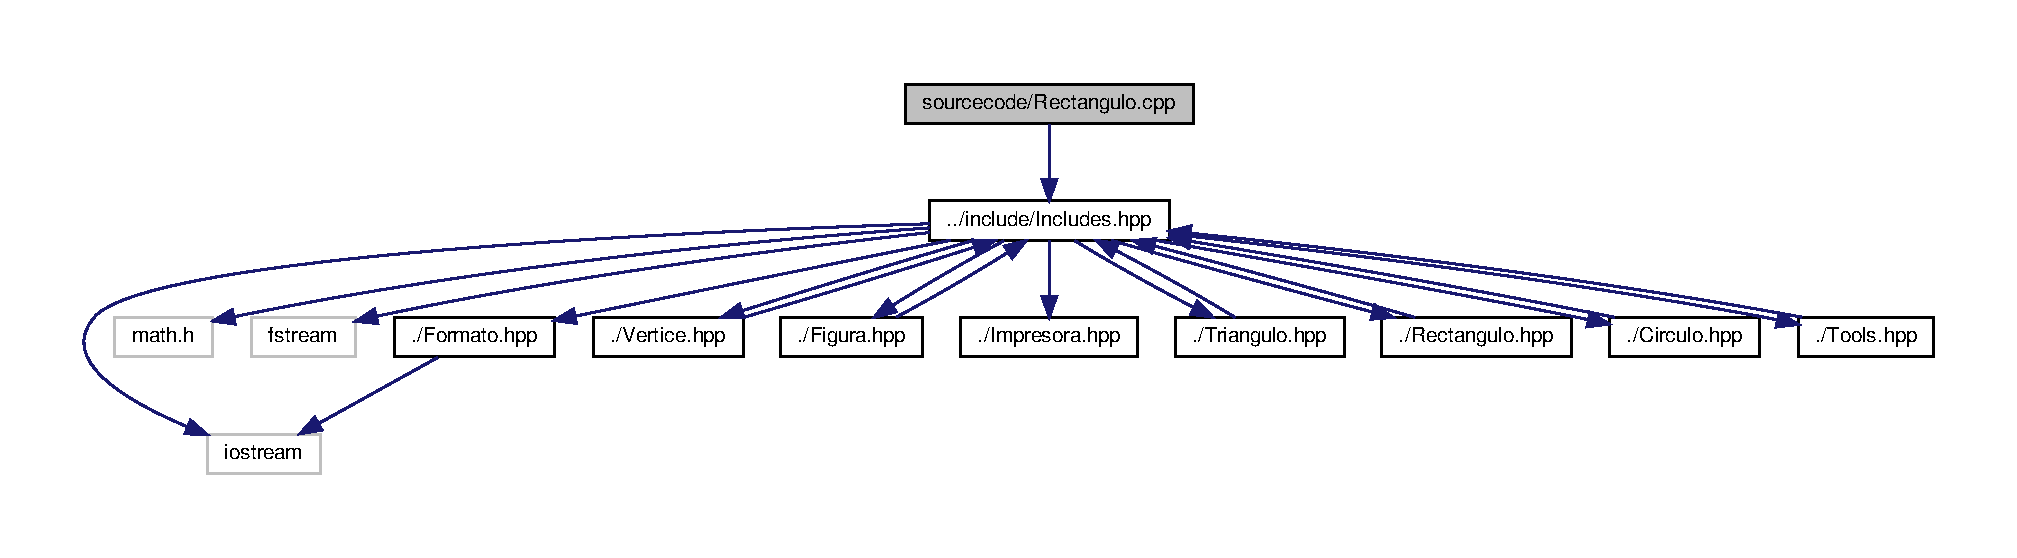
\includegraphics[width=350pt]{_rectangulo_8cpp__incl}
\end{center}
\end{figure}


\subsection{Detailed Description}
/ 
\hypertarget{_triangulo_8cpp}{}\section{sourcecode/\+Triangulo.cpp File Reference}
\label{_triangulo_8cpp}\index{sourcecode/\+Triangulo.\+cpp@{sourcecode/\+Triangulo.\+cpp}}
{\ttfamily \#include \char`\"{}../include/\+Includes.\+hpp\char`\"{}}\newline
Include dependency graph for Triangulo.\+cpp\+:
\nopagebreak
\begin{figure}[H]
\begin{center}
\leavevmode
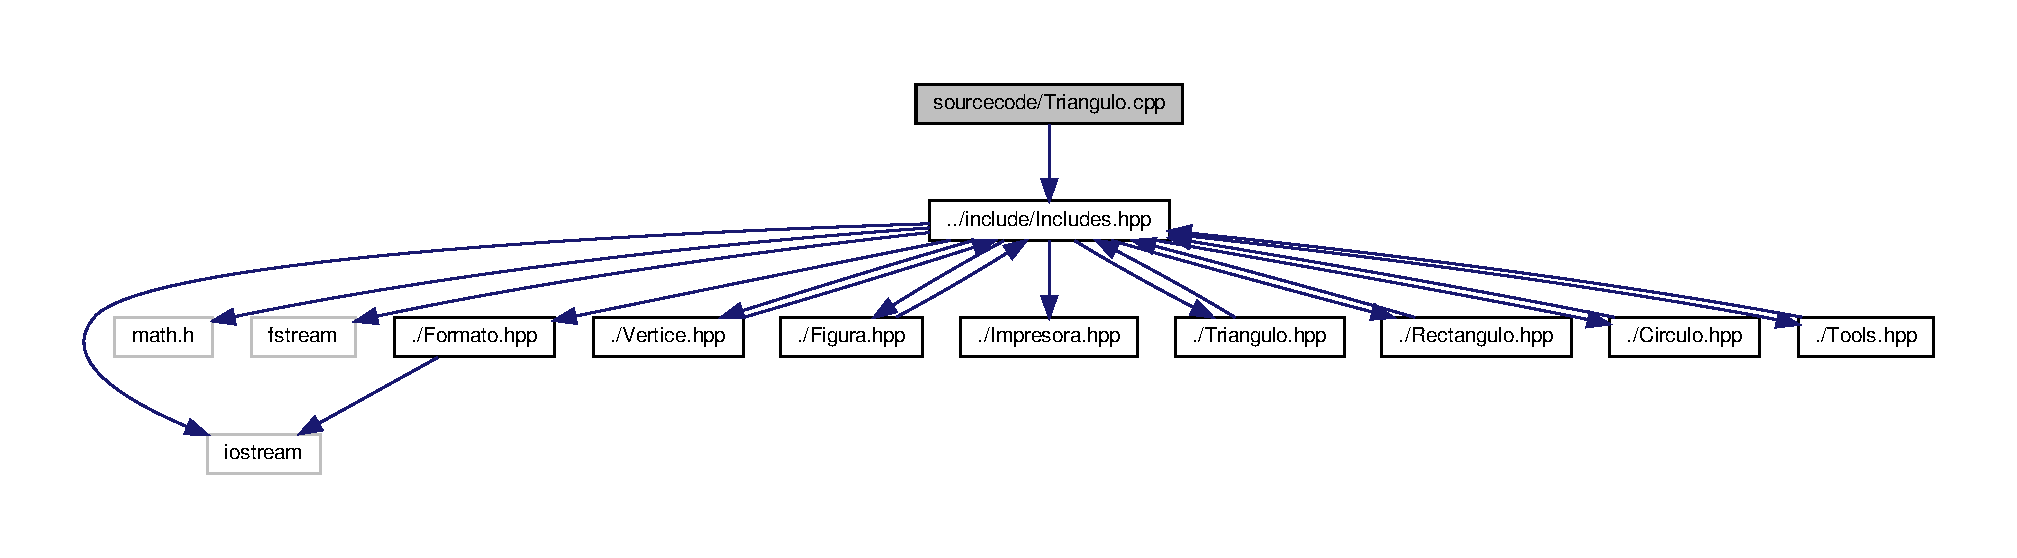
\includegraphics[width=350pt]{_triangulo_8cpp__incl}
\end{center}
\end{figure}


\subsection{Detailed Description}
/ 
\hypertarget{_vertice_8cpp}{}\section{sourcecode/\+Vertice.cpp File Reference}
\label{_vertice_8cpp}\index{sourcecode/\+Vertice.\+cpp@{sourcecode/\+Vertice.\+cpp}}
{\ttfamily \#include \char`\"{}../include/\+Includes.\+hpp\char`\"{}}\newline
Include dependency graph for Vertice.\+cpp\+:
\nopagebreak
\begin{figure}[H]
\begin{center}
\leavevmode
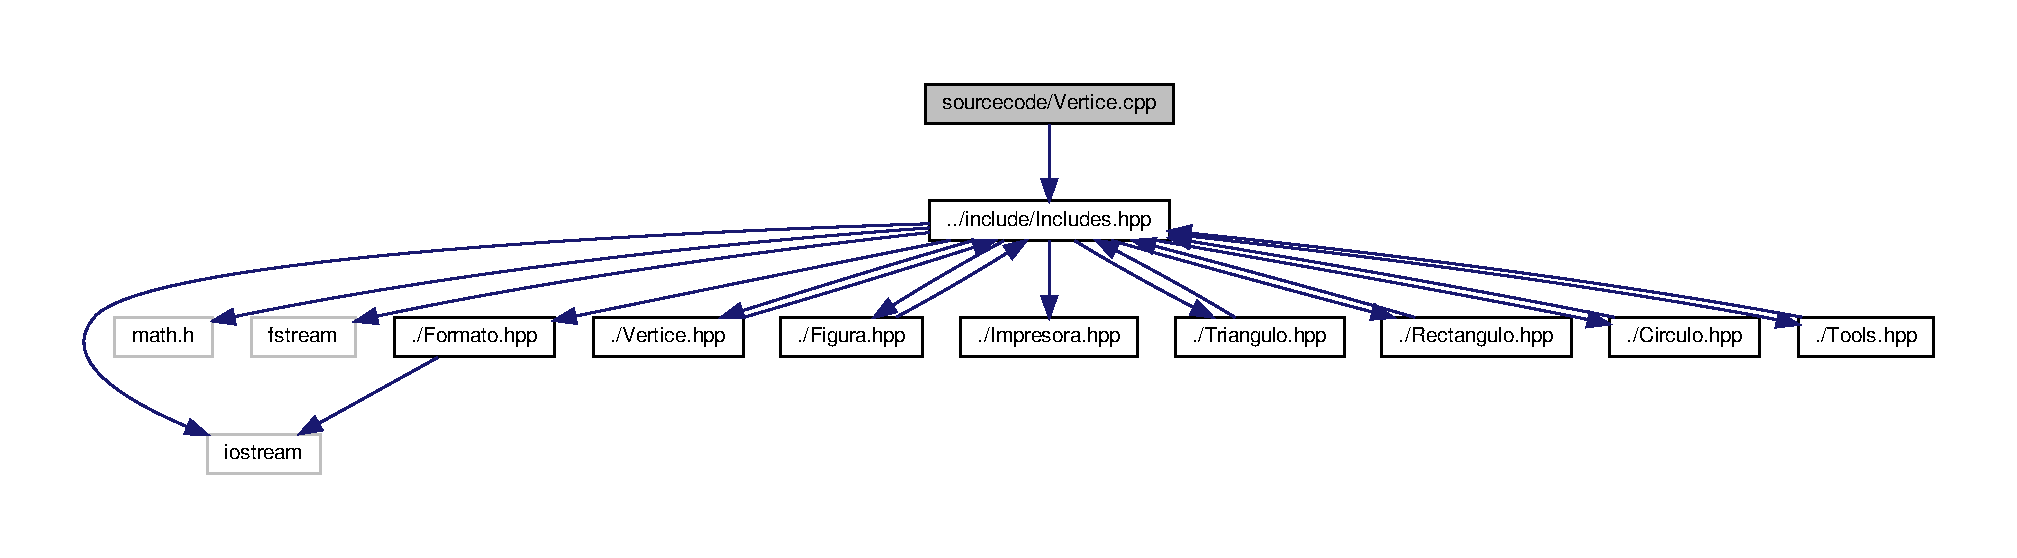
\includegraphics[width=350pt]{_vertice_8cpp__incl}
\end{center}
\end{figure}


\subsection{Detailed Description}
/ 
%--- End generated contents ---

% Index
\backmatter
\newpage
\phantomsection
\clearemptydoublepage
\addcontentsline{toc}{chapter}{Index}
\printindex

\end{document}
